% 4022 Project Thesis Template
% University of Cape Town Department of Electrical Engineering
% Template Version 0.1 - August 2021
% Adapted from the following 2 sources by J Wyngaard
% https://code.engineering.queensu.ca/ece/thesis-template-for-latex
% https://github.com/jpt13653903/LaTeX_UCT_Report.git

% NOTES TO USER:
% You should not need to edit this file (aside from section "TITLE PAGE"). Edit the individual files that are loaded. 
% For example, where you see \include{3_Preface/0_Preface/0_Abstract}, this loads your abstract from the file at Thesis/3_Preface/0_Preface/0_Abstract.tex. Open the file 0_Abstract.tex and edit.

% -> FILE DESCRIPTION :: Thesis.tex
%	This is the master file for your write-up.  It will combine all of the files together to create your thesis (Thesis.pdf). 

%	Thesis.tex will perform the following actions:
%	 1) Import all the supplemental packages
%	 2) Set the styling for the document
%	 3) Combine the various chapters, sections and other components of your thesis into one document.
%	 4) Create LaTex generated sections, such as Table of Context, Glossary, and Bibliography  

%*************************************************************************************************************
% DO NOT MODIFY:
%*************************************************************************************************************

% !TeX root = ../Thesis.tex
% 4022 Project Thesis Template
% University of Cape Town Department of Electrical Engineering
% Template Version 0.1 - August 2021
% Adapted from the following 2 sources by J Wyngaard
% https://code.engineering.queensu.ca/ece/thesis-template-for-latex
% https://github.com/jpt13653903/LaTeX_UCT_Report.git

% -> FILE DESCRIPTION :: Preamble.tex
%	This files defines the imports necessary for proper compiling of the thesis document and create the styling of the document.

%*************************************************************************************************************
% DOCUMENT
%*************************************************************************************************************
% -> This section defines the basic thesis document. 

% Set Document Type
\documentclass[12pt]{report}  

% Select Thesis Package
\usepackage{0_Config/1_Styles/UCT_EE_Thesis_Style}
    
%*************************************************************************************************************
% PATCHING
%*************************************************************************************************************
% -> This section imports functionality which fixes Latex bugs

% Modern LaTeX provides enough output streams without the legacy morewrites
% compatibility package, which can corrupt deferred writes during shipout.

%*************************************************************************************************************
% SPACING
%*************************************************************************************************************
% -> This section defines the basic spacing options for the thesis document. 

\usepackage{parskip} % Block paragraphs: no first-line indent, a blank gap between paragraphs instead

\usepackage{pgfplots}
\pgfplotsset{compat=1.18}
\usepackage{float}
\usepackage{rotating}
\usepackage{tikz}
\usetikzlibrary{
    arrows.meta,
    positioning,
    shapes.geometric,
    fit,
    backgrounds
}

%*******************************************************************************
% HEADINGS
%*******************************************************************************
% -> This changes the headings go that they are prettier, this can be commented out for traditional headings.

\usepackage{sectsty}

%*************************************************************************************************************
% FONTS
%*************************************************************************************************************
% -> This section defines the fonts for various document entities.

\allsectionsfont{\bfseries}% set all the section font to bfseries
\chapterfont{\Huge} % set the sizes of chapters, sections ...
\sectionfont{\Large}
\subsectionfont{\large}

%*************************************************************************************************************
% FORMATTING
%*************************************************************************************************************
% -> This section defines formatting Table of Contents entr
% example: Chapter 1 Introduction

\usepackage[subfigure]{tocloft}
\usepackage{tocloft}
\usepackage{multicol}

\renewcommand{\cftchappresnum}{Chapter }
\renewcommand{\cftchapaftersnum}{:}
\renewcommand{\cftchapnumwidth}{7em}

% for formatting Table of Contents entry for Appendix, example: Appendix 1: Stuff
\newcommand*\updatechaptername{%
   \addtocontents{toc}{\protect\renewcommand*\protect\cftchappresnum{Appendix }}
}

%*******************************************************************************
% FOOTNOTES
%*******************************************************************************
% -> This section defines formating for footnotes

\interfootnotelinepenalty=10000 % This line stops footnotes from splitting onto two pages.

%*******************************************************************************
% VERBATIM
%*******************************************************************************
% -> 

\usepackage{moreverb}        % Using this package to get better control of the
                             % verbatim environment, mostly for the use of the
                             % listing environment which puts line number
                             % beside each line.  Note that there has to be a number
                             % in each set of brackets, i.e., \begin{listing}[1]{1}.
                             % PDF info file is "The moreverb package" by
                             % Robin Fairbairns (rf@cl.cam.ac.uk) after
                             % Angus Duggan, Rainer Schopf and Victor Eijkhout, 2000/06/29.
%-------------------------------------------------------------------------------
%\usepackage{verbatim}        % allows the use of \begin{comment} and \end{comment}
                             % as well as \verbatiminput{file}
                             % Note:  when using verbatim to input from a text file,
                             % such as a specification or code, use \begin{singlespacing}
                             % and \end{singlespacing}.  Also, tabs are not read
                             % properly, so the input file must only use spaces.

%                             \begin{comment}
%                             Can also use the verbatim package for
%                             comments like this...
%                             \end{comment}


%*******************************************************************************
% GLOSSARY
%*******************************************************************************
% -> Creates the glossary

\usepackage[acronym,automake,toc]{glossaries}
\newglossary[slg]{symbol}{sym}{sdn}{List of Symbols}
\makeglossaries

% See Glossary/Glossary.tex for the content of your glossary

%*******************************************************************************
% INDEX
%*******************************************************************************
% -> Creates the Index

\usepackage{makeidx}         
\makeindex

%*******************************************************************************
% MATH
%*******************************************************************************
% -> Import and configure packages for math
\usepackage{mathrsfs}		 % For Symbols
\usepackage{amssymb}		 % For More Symbols
\usepackage{amsfonts}		 % For Other Symbols
\usepackage{amsmath}         % For Equations
\usepackage{amsthm}          % For Theorems & Definitions


% Using the amsthm package, define a new theorem environment for my
% definition.  * means don't number it.
\newtheorem*{definition}{Definition}
\usepackage{cases}           % to make numbered cases (equations)
\usepackage{calc}            % Used with the Ventry environment defined below.

%*******************************************************************************
% FLOATS, PLOTS, AND FIGURES
%*******************************************************************************
% -> This section defines and configures packages for various styles of floating objects and figures. 
 
\usepackage{graphicx}       % for graphic images (use \includegraphics[...]{file.eps})
%\usepackage{subfigure}      % for subfigures (figures within figures)
\usepackage{subfig}			% for subfigures (figures within figures). Same as subfigures except it works.
\usepackage{wrapfig}		% for wrapping text around figures
%\usepackage{boxedminipage}  % to make boxed minipages, i.e., boxes around figures
\usepackage{rotate}         % for use of \begin{sideways} and \end{sideways}
\usepackage{listings}       % for use of printing code blocks
\usepackage{pgfplots}		% for plots
\usepackage{pdfpages}		% for importing PDFs
\usepackage[normalem]{ulem}

%*******************************************************************************
% CUSTOM FORMATTING
%*******************************************************************************

\usepackage[table]{xcolor}
\usepackage{geometry}
\geometry{
    a4paper,
    left=25mm,
    right=25mm,
    top=25mm,
    bottom=25mm,
    headheight=15pt,
    headsep=7mm,
    footskip=10mm
}


%*******************************************************************************


% Define how the ``listings'' to look.
%\lstset{basicstyle=\footnotesize,, numbers=left, numberstyle=\small, stepnumber=1, numbersep=5pt, showspaces=false, lineskip=-1pt}

\usepackage{float}           % Using this package to get better control of floats
                             % including the ability to define new float types for
                             % specification and code listings.
                             % DVI info file is "An Improved Environment for Floats"
                             % by Anselm Lingnau, lingnau@tm.informatik.uni=frankfurt.de
                             % 1995/03/29.

% Style of float used for code listings
\floatstyle{ruled}
\newfloat{Listing}{H}{lis}[chapter]
\renewcommand{\lstlistlistingname}{List of Code Listings} % Title be changed as necessary

                             % Note:  The listings don't have space between the chapters, unlike
                             % the standard list of tables etc.  At the end, copy the spacing
                             % commands from the .toc file and insert into the .lis file.  Then,
                             % DO NOT LATEX it again, simply go to the DVI viewer!

\usepackage{placeins} % for \FloatBarrier which stops floats from crossing a point

%*******************************************************************************
% TABLES
%*******************************************************************************
% -> This section defines tables
\usepackage{booktabs}

\usepackage{array}
\usepackage{tabularx}        % Package used to make variable width-columns, i.e.,
                             % column widths are changed to fit the maximum width
                             % and text is wrapped nicely.

\usepackage{threeparttable}

\usepackage{lscape}			% For landscape
\usepackage{adjustbox}		% To adjust table width
\usepackage{multirow}		% For merging and splitting table cells

%*******************************************************************************
% CAPTIONS
%*******************************************************************************
% ->  This section defines captions

\usepackage{caption}   % Package used to make my captions 'hang', i.e., wrap around, but not under the name of the caption.
%\usepackage[justification=centering]{caption} % Captions that are centered
                             

% Find that the captions are too far from my verbatim figures, but if
% I change it to 0, then the captions are too close for my other types
% of figures.  Maybe set each one separately?
%\setlength{\abovecaptionskip}{1ex}

%\setlength{\textfloatsep}{1ex plus1pt minus1pt}

%\setlength{\intextsep}{1ex plus1pt minus1pt}

%\setlength{\floatsep}{1ex plus1pt minus1pt}

%*******************************************************************************
% MISCELLANEOUS
%*******************************************************************************
% ->  This section defines miscellaneous packages that facilitate miscelaneous things

\usepackage{layout}          % useful for determining the margins of a document
                             % use with \layout command
                             
\usepackage{changebar}       % Way of indicating modifications by putting bars in the
                             % margin.  Read about it in "The Latex Companion".
                             
\usepackage{enumitem}		% For enumerated lists

%*******************************************************************************
% REFERENCES ETC.
%*******************************************************************************
% ->  This section defines the reference section

\usepackage{varioref}        % Better page references, e.g., "on preceding page", etc.
                             % \vref{key} Create an enhanced reference.
                             % \vpageref[text]{key} Create an enhanced page reference.
                             % \vrefrange{key}{key} Create an enhanced range of references.
                             % \vpagerefrange[text]{key}{key} Create an enhanced range of page references.
                             % Note: doesn't really work for consecutive pages.

% Renewing the text for before and after
\renewcommand{\reftextafter}{on the next page}
\renewcommand{\reftextbefore}{on the previous page}
\usepackage{url}             % for use of \url - pretty web addresses
\usepackage{fancyhdr}
\usepackage{cite}
\usepackage{notoccite}      % Prevents references from starting in TOC, List of Figures, etc.

%*******************************************************************************
% Block Diagrams
%*******************************************************************************
% ->  This section defines imports for block diagrams and flow charts

\usepackage{tikz}
\usetikzlibrary{arrows,automata,arrows.meta}

% Block Diagram
\tikzstyle{block} = [draw,fill=blue!20,minimum size=2em]
\def\radius{.7mm} 
\tikzstyle{branch}=[fill,shape=circle,minimum size=3pt,inner sep=0pt]

% Flow Charts
\usepackage{pgf}
\usepackage[utf8x]{inputenc}
\usetikzlibrary{positioning,calc}
\tikzset{
	state/.style={
		rectangle,
		rounded corners,
		draw=black, very thick,
		minimum height=2em,
		inner sep=2pt,
		text centered,
	},
}

%*******************************************************************************
% HYPERLINKS (must be last)
%*******************************************************************************
% ->  This section defines how hyperlinks function

% Uncomment these next two lines for linkback to citation pages in biblio
%%#\renewcommand*\backref[1]{\ifx#1\relax \else \linebreak Cited on page(s): #1. \fi}

\hypersetup{
	colorlinks=true,  % Change links to being coloured text, no boxes
	linkcolor=blue,
	urlcolor=blue,
    citecolor=blue
}
% Neat package to turn href, ref, cite, gloss entries
% into hyperlinks in the dvi file.
% Make sure this is the last package loaded.
% Use with dvips option to get hyperlinks to work in ps and pdf
% files.  Unfortunately, then they don't work in the dvi file!
% Use without the dvips option to get the links to work in the dvi file.

% Note:  \floatstyle{ruled} don't work properly; so change to plain.
% Not as pretty, but functional...
% The bookmarks option sets up proper bookmarks in the pdf file :)

% Need this command to allow hyperref to play nicely with gloss; otherwise
% almost every \gloss will cause an error...
%%#\renewcommand{\glosslinkborder}{0 0 0}

\usepackage[colorinlistoftodos]{todonotes}
\newcommand{\todoall}[1][]{\todo[color=yellow, inline]}

%*******************************************************************************
% CUSTOM CHAPTER SPACING
%*******************************************************************************

\makeatletter

\renewcommand{\@makechapterhead}[1]{%
  \vspace*{0pt}%
  {\parindent \z@ \raggedright \normalfont
    \ifnum \c@secnumdepth >\m@ne
        \huge\bfseries \@chapapp\space \thechapter
        \par\nobreak
        \vskip 10pt
    \fi
    \interlinepenalty\@M
    \Huge\bfseries #1\par\nobreak
    \vskip 20pt
  }}

\renewcommand{\@makeschapterhead}[1]{%
  \vspace*{0pt}%
  {\parindent \z@ \raggedright \normalfont
    \interlinepenalty\@M
    \Huge\bfseries #1\par\nobreak
    \vskip 20pt
  }}

\makeatother

\begin{document}

%*************************************************************************************************************
% TITLE PAGE 
%	INSERT THE DETAILS OF YOUR THESIS
%	REMOVE THE '%' TO UN-COMMENT LINE
%*************************************************************************************************************
\makeatletter
\title{Design and development of a smart sunbird feeder for autonomous video-based behavioral monitoring}\let\Title\@title
\author{Jack Youens}            \let\Author\@author
\makeatother

\supervisor{Yaaseen Martin}
\dept{Electrical Engineering}
\degree{Mechatronic Engineering}
\copyrightyear{2026}

\beforepreface

%*******************************************************************************
% ABSTRACT
%*******************************************************************************
\phantomsection
\prefacesection{Abstract}

% INSERT YOUR ABSTRACT %

In the ever-growing field of automated bird monitoring and identification, the range of cost-efficient and non-invasive methods for ecological monitoring of species of birds is wanting. The aim of this project is to investigate the design and implementation of a smart sunbird feeder capable of detecting and identifying nectar-feeding birds using an embedded ML algorithm coupled with a computer-vision system while remaining affordable. The system used was trained to recognize 22 species of birds with a focus on the 6 nectar-feeding species known to reside in the Cape Town area. Across these species, the system achieved an accuracy of \_\_\_ in identifying the species correctly and achieved an average inference time of \_\_\_. These results demonstrate the feasibility of using a targeted, low-cost smart feeder as an automated monitoring system and provide a basis for more efficient collection of species-level visitation data in future ecological studies.

%--------------------------------------------------------------------
% Taken from "Scientific Writing by D. Branch Moody"
%--------------------------------------------------------------------
% The abstract is 2 to 6 sentences long and is always less than 500 
% words.  Abstracts are increasingly less than 200 words, 
% according to journal rules. The abstract outlines three points: 
% the field's gap in knowledge, the outcomes of experiments and their
% impact on the field. 
%
% In learning to write abstracts for national meetings, you were 
% probably taught to include descriptions of individual experiments 
% and methods.  The "national meeting" abstract is your only 
% chance to communicate results to the reviewers, so is longer 
% and more detailed.
%
% The abstract submitted to a journal for publication is 
% immediately followed by all of the experiments, so the abstract 
% itself does not need to list every finding and method.  Thus, an  
% abstract for a paper submitted to a journal is usually more 
% conceptual and clearly states the take home point. Increasingly,
% journals have shortened the allowed length of abstracts with 
% many now in the range of 100 to 200 words. Journals now strongly
% encourage authors to focus on the conceptual advance rather 
% than the serial of listing individual experiments. Readers are
% usually interested in why the work is new and important and 
% not a detailed listing of the mouse strains and monoclonal
% antibodies used. 
%
% 'Current knowledge ends' statement. Experienced writers are 
% careful to say where knowledge ends in a statement that comes 
% before the explanation of the new data starts.  The "current 
% knowledge ends" statement, if well crafted, will make it self 
% evident how the new data in the submitted is original or important.
% For example, the second sentence of an abstract could say 
% "Current knowledge of human CD1-reactive T cells derives mainly 
% from study of individual T cell clones, but the roles of such 
% T cell in vivo are not known."  This creates the general 
% expectation that the data that follow are opening up new avenues, 
% yet still allows the reader to decide if the point is proven. 
%--------------------------------------------------------------------   

%*******************************************************************************
% ACKNOWLEDGEMENTS
%*******************************************************************************
\phantomsection
\prefacesection{Acknowledgements}

% INSERT YOUR ACKNOWLEDGEMENTS %
%I would like to acknowledge my parents and friends. This thesis, a manifestation of the many sleepless nights, would not have been possible without their support. This section highlights your acknowledgment of individuals whom you believe deserve recognition for their contribution towards making your achievement possible.  

\clearpage % keep this for proper page numbering!   

%*******************************************************************************
% PLAGIARISM DECLARATION
%*******************************************************************************
\phantomsection
\prefacesection{Plagiarism Declaration}

    \begin{enumerate}
        \item I know that plagiarism is wrong. Plagiarism is to use another's work and pretend that it is one's own.
        \item I have the IEEE convention for citation and referencing. Each contribution to, and quotation in, this final year project report from the work(s) of other people, has been attributed and has been cited and referenced.
        \item This final year project report is my own work.
        \item I have not allowed, and will not allow, anyone to copy my work with the intention of passing it off as there own work or part thereof.
    \end{enumerate}

    \vspace{15mm}

    \mbox{}\hfill\begin{minipage}{65mm} % No need to change this part
      \dotfill\\[1ex]%
      \Author\\
      \today
    \end{minipage}
    
    \vfill\vfill\vfill

   

%*******************************************************************************
% Table of Contents
%*******************************************************************************
% Print the Table of Contents 
\PageContentstrue

% To disable, use the following:
%\PageContentsfalse

%*******************************************************************************
% The following lists can be commented out if not necessary for your thesis:
%*******************************************************************************

%*******************************************************************************
% Glossary
%*******************************************************************************
% The Glossary 
\PageGlossariestrue

% To disable, use the following:
%\PageGlossariesfalse

% Include Glossary
% -> FILE DESCRIPTION :: Glossary.tex
%	This files contains all of your glossaries. It has been configured to have your main glossary (definitions), acronym glossary and symbols glossary.

% ---------------------------------------------------------------------------------------------%

% MAIN (Definitions) GLOSSARY
% \newglossaryentry{NameInLink}{
%	name={NameToShow},
%	sort=NameInSort,
%	description={What does it mean?}
%	}

\newglossaryentry{diction}
{
	name={diction},
	sort=diction,
	description={the choice and use of words and phrases in speech or writing}
}
\newglossaryentry{lexicon}
{
	name={lexicon},
	sort=lexicon,
	description={the vocabulary of a person, language, or branch of knowledge}
}

\newglossaryentry{prose}
{
	name={prose},
	sort=prose,
	description={written or spoken language in its ordinary form, without metrical structure}
}
\newglossaryentry{ADC}
{
	name={ADC},
	sort=ADC,
	description={Analogue-to-Digital Converter}
}

% ---------------------------------------------------------------------------------------------%

% ACRONYMS
% \newacronym{NameInSort}{NameToShow}{Definition}
\newacronym{lol}{LOL!}{Laugh Out Loud}


% ---------------------------------------------------------------------------------------------%

% SYMBOLS
% \newglossaryentry{NameInLink}{
%	type=symbol, 
%	name={NameToShow},
%	sort=NameInSort,
%	description={What does it mean?}
%	}

\newglossaryentry{mySymbol}{
	type=symbol,
	name={\textrm{$\Upsilon$}},
	sort=thresh,
	description={Arbitrary symbol.}
}



% This line forces all entries into glossary, even if they have not been referenced
% UNCOMMENT THIS LINE TO INCLUDE ALL GLOSSARY ITEMS (Not just those referenced)
% \glsaddall

% UNCOMMENT INDIVIDUAL GLOSSARIES TO BE PRINTED (IF not using \PageGlossariestrue) %
% \printglossaries % Prints ALL glossaries.
% \printglossary % Print the terms glossary
% \printglossary[title = Nomenclature] % Print the terms glossary
% \printglossary[type=symbol, title=List of Symbols] % Prints the acronym glossary
%\printglossary[type=\acronymtype,title=Glossary of Abbreviations] % Prints the abbreviation glossary

%*******************************************************************************
% List of Tables
%*******************************************************************************
% Print the List of Tables
\PageTablestrue

% To disable, use the following:
%\PageTablesfalse

%*******************************************************************************
% List of Figures
%*******************************************************************************
% Print the List of Figures
\PageFigurestrue

% To disable, use the following:
%\PageFiguresfalse


%*******************************************************************************
% List of Code Snippets
%*******************************************************************************
% Print the List of Code Snippets
%\PageCodeSnippetstrue

% To disable, use the following:
\PageCodeSnippetsfalse

%*******************************************************************************
% List of Equations
%*******************************************************************************
% Print a list of all equations
%\PageEquationstrue

% To disable, use the following:
\PageEquationsfalse

%*******************************************************************************
% Apply Apply After Preface - DO NOT MODIFY
%*******************************************************************************
% Create afterpreface sections
\afterpreface


%*******************************************************************************
% 0.7 - CHAPTERS
%*******************************************************************************
% Include Chapters. Chapters are kept separated to make editing easier.

% Chapter 1 - Introduction

\glsresetall % reset the glossary to expand acronyms again
\chapter[Introduction]{Introduction}\label{ch:Introduction}
\index{Introduction}

% Background
\section{Background}

Birds are integral members of our ecosystems as providers of many roles that prove vital to the health of these ecosystems, be they predators, pollinators, scavengers, seed dispersers, seed predators, or ecosystem engineers \cite{Whelan2008}. Sunbirds in particular have proven to be especially important in the pollination process and are a dominant group of nectar feeders throughout Africa. In the Western Cape specifically, sunbirds have been found to be the primary pollinators of several plant species \cite{deWaal2012}. Furthermore, in Cape Town nectarivorous birds have been established to play an unusually important role in the ecosystem due to the highly asymmetrical mutual pollination between birds and plants in this biodiversity hotspot \cite{Coetzee2018}. Despite their integral ecological role, however, the capturing of data of when, how often and what species of this group interact with particular food sources remains a challenging task. The current means of obtaining these measurements are time-consuming and are heavily dependent on human labour. These factors have led directly to practical limitations on the monitoring of these birds.
\par\vspace{6pt}
More recently, camera traps have become a much more efficient means of remotely capturing animal distribution, abundance and behaviour, but this method of ecological monitoring remains limited by sampling errors such as false triggers and data extraction from this footage is still an expensive, time-consuming and manual task \cite{Burton2015, Norouzzadeh2018}. With advancements in the fields of digital imaging, embedded computing and computer vision, automatic and remote ecological monitoring becomes a much more feasible option while simultaneously reducing the amount of false detection instances \cite{Christin2019}. Already, machine learning has been proven able to identify animals from camera trap footage with a highly reliable accuracy \cite{Norouzzadeh2018}. Such developments make possible a compact and cost-effective method of not only collecting data for ecological monitoring, but doing so intelligently with minimal or no requirement of human intervention.
\par\vspace{6pt}
The monitoring of nectarivorous birds is made much more viable at known hotspots of nectarivore activity such as feeding sites. Introducing a nectar feeder to a nearby feeding location is a sound method of localizing bird activity to a well-constrained area as well as standardizing an angle of captured footage, since the feeding port requires these birds to perch on a specific platform. Recent studies have proven the viability of embedded machine learning algorithms in detecting and monitoring avian sightings at feeder stations \cite{Youngblood2019}. An adapted system for nectar-feeding birds that similarly incorporates video monitoring, automated feeder visit detection and species identification could prove to contribute significantly to the available monitoring methods of these birds.

\section{Problem Statement}

Sunbirds are difficult creatures to monitor. They are small, highly mobile and easily disturbed. Current aviary monitoring methods have shown that a combination of camera recording, embedded computing and machine learning makes automated monitoring viable. 
\par\vspace{6pt}
Analysis of current projects expose an engineering gap that this project will aim to fill. There is a need for a compact and reliable system designed to cater specifically to nectar feeding birds and their physical behaviour while being capable of unsupervised operation, reliable footage capture with associated species predictions and sufficient off-grid capacities.

\par\vspace{6pt}
Existing Technology includes:
\begin{itemize}
    \item Camera-equipped smart feeders
    \item Raspberry Pi/embedded wildlife-monitoring systems
    \item Motion/event-triggered image or video capture
    \item Machine-learning species classification
    \item Solar-powered monitoring systems
\end{itemize}

\par\vspace{6pt}
Limitations of existing technology are:
\begin{itemize}
	\item Designed around seed feeders or hummingbird-style products
    \item Dependent on external/cloud infrastructure in some cases
    \item Not specifically designed around local South African nectar-feeding birds
    \item Not optimised for low-power autonomous field operation
\end{itemize}

Considering this engineering gap in the field of automated bird monitoring as well as the relevant existing technology and its limitations, the following problem statement for this project was defined:

\section{Objectives}

This project aims to design and deploy an autonomous and remote smart nectar feeder, with a primary focus on monitoring sunbirds in the Cape Town area. The system will utilise a machine learning algorithm locally embedded on an edge processing device to classify classes of interest and record visits of such classes. These recordings will be made available to users via a locally-hosted web interface. 
\par\vspace{6pt}
For the objectives of this project to be achieved, a functional prototype of the complete system must be developed, assembled and tested in the field. The objectives this project aims to achieve through the realisation of a successful prototype include:

\begin{itemize}
  \item Designing and constructing a nectar feeder arrangement suitable for sunbirds and camera monitoring
  \item Developing an automated system for detecting bird visits
  \item Capturing video footage of detected visits
  \item Implementing embedded species classification using a locally relevant dataset
  \item Storing video recordings and their associated observation metadata locally
  \item Developing an autonomous power system using battery and solar energy
  \item Integrating the subsystems into an deployable prototype
  \item Evaluating detection, classification, video, power and overall system performance
\end{itemize}

\section{Scope and Limitations}
The scope of this project defines the functional and technical boundaries within which the smart sunbird feeder will be designed, implemented and evaluated. These boundaries are intended to keep the project focused on the development of a reliable and practical monitoring system, while acknowledging constraints associated with time, resources, deployment conditions and system capability. The scope of this project is set as follows:
\begin{itemize}
\item \textbf{Hardware scope:} Data collection will use a Raspberry Pi, a single camera module and a single Time-of-Flight (ToF) sensor.
\item \textbf{Time scope:} Monitoring will be limited to daytime bird activity.
\item \textbf{Subject scope:} The system will focus on sunbirds and other relevant nectar-feeding bird species.
\item \textbf{Monitoring scope:} Bird visits will be recorded using motion-triggered capture rather than continuous monitoring.
\item \textbf{Location scope:} System deployment and evaluation will be limited to Cape Town.
\item \textbf{Data scope:} Captured data will consist of a short video recording, the predicted species and corresponding confidence score, and the date and time of the observation.
\item \textbf{Storage scope:} All captured data will be stored locally on the system.
\item \textbf{Ethics scope:} Species classification and monitoring will be conducted using entirely non-invasive methods.
\end{itemize}

Similarly, the limitations of this project are defined as follows:

\begin{itemize}
\item \textbf{Hardware limitation:} The project is limited to adapting a commercially available nectar feeder and integrating existing electronic components. Custom PCB design and development of new circuitry will not be undertaken.
\item \textbf{Species limitation:} Only bird species relevant to South Africa will be considered as classes of interest. Foreign species will not be included.
\item \textbf{Classification limitation:} Classification will be limited to species level. Sex, age and individual identification will not be considered.
\item \textbf{Data collection limitation:} Bird behaviour will not be analysed. Collected data will be limited to species identification, the date and time of each visit, and an accompanying video recording.
\item \textbf{Time limitation:} The project must be completed by 26 October 2026.
\item \textbf{Budget limitation:} The project is constrained to a budget of R2000.
\item \textbf{Energy limitation:} Solar-energy generation is dependent on environmental conditions, particularly solar irradiance and cloud cover.
\item \textbf{User interface limitation:} User interaction with collected data will be limited to a simple, locally hosted web interface. Development of a dedicated desktop or mobile application will not be considered.
\end{itemize}

% Thesis Outline
\section[Outline]{Thesis Outline}
The remainder of this thesis is organized as follows:\\
\textbf{Chapter 2, Background:} Background and literature review\\
\textbf{Chapter 3, Methodology:} Project methodology\\
\textbf{Chapter 4, Design:} Design and development\\
\textbf{Chapter 5, Results:} Experimental results\\
\textbf{Chapter 6, Conclusions:} Conclusions and future work
% Chapter 2 - Background

\glsresetall % reset the glossary to expand acronyms again
\chapter[Literature Review]{Literature Review}\label{ch:LitReview}
\index{Literature Review}

% Literature Review
%\section{Literature Review}

\section{Introduction}

%\begin{itemize}
%    \item \sout{Purpose/scope of lit review. }
%    \item \sout{Areas of lit reviewed. }
%    \item \sout{How the lit review will impact the design.} 
%    \item Boundaries of lit review.
%\end{itemize}
The purpose of this literature review is to survey and investigate relevant literature to aid the design of a smart sunbird feeder. The literature reviewed will inform subsequent design choices and methods. Literature concerning ecological and avian monitoring will support the motivation for research in this area, while identifying sunbird behaviours and characteristics of nectar feeders that may present difficulties or limitations. Existing automated bird-monitoring solutions will be analysed to determine how aspects of similar research can best be applied. Several key enabling technologies will then be investigated, together with their respective advantages and disadvantages. Finally, the literature review will identify important trade-offs in similar projects and address the research gap this project aims to fill. The findings will support informed design and implementation decisions based on the accomplishments and limitations reported in the literature.

\section{Bird monitoring and nectarivorous ecology:}

%\begin{itemize}
%    \item \sout{Importance of monitoring bird activity.}
%    \item \sout{Normal monitoring methods and their limitations.}
%    \item \sout{Benefits of non-invasive monitoring.} 
%    \item \sout{A bit of relevant sunbird behaviour.} 
%    \item \sout{Unique aspects of nectar feeders.} 
%    \item \sout{Ecology/hygiene issues around supplemental feeding.}
%\end{itemize}

Firstly, it is important to establish the relevance of ecological monitoring as motivation for research in this field, which this section aims to accomplish.
\par\vspace{6pt}
Bird activity is a vital metric for determining ecosystem biodiversity and functioning. Nations have adopted methods of observing this activity to support sustainable development strategies and gauge environmental and ecosystem health \cite{GregoryVanStrien2010}. Conventional avian ecological monitoring includes approaches such as human point counts, passive sound recording and camera traps. These methods have proven practically identical in effectiveness when implemented correctly, while remote observation is preferred for remote deployment or rare species monitoring \cite{DarrasEtAl2018}. Sound recording and similar autonomous methods reduce the time required for human monitoring, provide permanent data capture and eliminate human observer bias. These methods also have drawbacks, including equipment and storage costs and the risk of data loss if they fail \cite{ShonfieldBayne2017}. Despite these shortcomings, remote monitoring systems, particularly camera traps, are widely used for wildlife monitoring. Depending on the model, set-up and application, camera traps are viable for a diverse range of scenarios \cite{TrollietEtAl2014}. \textbf{The advantages, limitations and project suitability of these monitoring methods are summarised in} Table~\ref{tab:birdmonitoringmethods}.

\begin{table}[htbp]
    \centering
    \caption{Comparison of common methods used for monitoring bird activity.}
    \label{tab:birdmonitoringmethods}
    
    \small
    \renewcommand{\arraystretch}{1.25}
    
    \begin{tabularx}{\textwidth}{
        >{\raggedright\arraybackslash}p{0.18\textwidth}
        >{\raggedright\arraybackslash}X
        >{\raggedright\arraybackslash}X
        >{\raggedright\arraybackslash}p{0.20\textwidth}
    }
        \toprule
        \textbf{Method}
        & \textbf{Principal advantages}
        & \textbf{Principal limitations}
        & \textbf{Suitability for this project} \\
        \midrule
        
        Human point counts
        & Can identify birds using both visual and acoustic observations; requires relatively little equipment; experienced observers can interpret behaviour and surrounding conditions immediately.
        & Requires trained observers and considerable field time; observations are restricted to scheduled survey periods; susceptible to observer bias; generally provides no permanent visual record.
        & Low. Useful for manually validating system observations, but unsuitable as the primary method for continuous autonomous monitoring. \\
        
        \addlinespace
        
        Passive acoustic monitoring
        & Enables long-duration unattended recording; provides a permanent record; can detect birds that are hidden from view; reduces the need for an observer to remain in the field.
        & Produces large volumes of audio data; performance is affected by background noise and overlapping calls; silent birds cannot be detected; reliable species identification may require specialist analysis or automated classifiers.
        & Moderate. Valuable for monitoring vocal activity, but it cannot provide the visual information required by the proposed image-based classification system. \\
        
        \addlinespace
        
        Camera-trap monitoring
        & Provides permanent visual records; enables verification of species, visit duration and aspects of behaviour; can operate autonomously; supports automated image or video analysis.
        & Detection depends on camera placement and trigger performance; false and missed activations may occur; image quality is affected by lighting, motion and occlusion; video requires substantial storage and energy.
        & High. The predictable feeding location allows the camera field of view and trigger region to be constrained, making this the most appropriate primary monitoring method. \\
        
        \bottomrule
    \end{tabularx}
    
    \vspace{0.5em}
    
    \begin{minipage}{0.96\textwidth}
        \footnotesize
        \textit{Sources:} Comparison informed by Darras et al. 
        \cite{DarrasEtAl2018}, Shonfield and Bayne 
        \cite{ShonfieldBayne2017}, and Trolliet et al. 
        \cite{TrollietEtAl2014}.
    \end{minipage}
\end{table}

\par\vspace{6pt}
In Cape Town, sunbirds have been shown to play a particularly important ecological role, with the four local nectar-feeding species contributing significantly to the maintenance of the region's many bird-pollinated plant species \cite{GeertsEtAl2020}. This role is accompanied by behavioural traits that affect how they should be monitored. Although sunbirds can hover while feeding, they frequently perch near nectar sources when an appropriate platform is available. Providing a perch therefore makes camera-based monitoring more practical \cite{SejfovaEtAl2021}. Sunbirds also associate food-source quality with colour, making feeder appearance more important than for seed-feeding species \cite{WhitfieldEtAl2014}. Many nectar feeders therefore use red feeding ports because red is common among flowers, highly visible in natural settings and less detectable to bees, reducing competition at the food source \cite{ChenEtAl2020}. Sunbird feeding routines also adapt to the location and quality of available food sources. Feeder activity should therefore not be assumed to represent overall sunbird activity in the surrounding area \cite{DuPlessisEtAl2021}. While some studies suggest supplemental feeding may concentrate sunbird activity and affect surrounding pollination networks, others report negligible effects on activity at natural food sources \cite{DuPlessisEtAl2021, MantintsililiEtAl2025}.
\par\vspace{6pt}
Sunbird feeders differ significantly from ordinary seed feeders because these birds are nectarivorous. Their diet requires feeders to contain liquid rather than solid food and, due to their long bills and "tube-like" tongues, they prefer narrow feeding ports over the trays commonly used in seed feeders \cite{CubanEtAl2026}. The nectar solution consists of water supplemented with sugar, particularly sucrose. Studies of sunbird feeder preferences found sucrose-rich solutions to be more popular than hexose-rich alternatives \cite{FlemingEtAl2004}. However, storing nectar in feeders can promote microbial transmission and fermentation, resulting in ethanol production. An analysis of hummingbird feeders found non-pathogenic bacteria and fungi that differed significantly from those found in flowers \cite{LeeEtAl2019}. Additionally, an ethanol concentration of only 2\% was found to significantly reduce sunbird visitation \cite{ChoiEtAl2023}. For these reasons, feeder nectar should be replaced regularly.

\section{Analysis of existing smart bird feeders}

%Focus on 
%\begin{itemize}
%    \item Intended purpose
%    \item Monitoring capabilities
%    \item Feeder type
%    \item Image or video capture
%    \item Species identification
%    \item Embedded operation
%    \item Connectivity and data access
%    \item Power supply
%    \item Outdoor deployment and reliability
%\end{itemize}

This section of the literature review will be dedicated to investigating the efforts of other individuals in similar fields of research and acknowledging the benefits and drawbacks for each of their respective approaches to conducting their research. 
\par\vspace{6pt}

\subsection{Research and experimental smart-feeder systems}
Rapid advances in Machine Learning (ML) and the increasing availability and affordability of microcomputers such as the Raspberry Pi (RPi) have enabled the development of smart bird feeders by both companies and academics. Researchers have demonstrated the feasibility of using an RPi as the computational core of a smart seed feeder, reliably capturing data from visiting birds using video, microphone and strain gauge recordings \cite{NiersEtAl2022}. The system also performed local species inference using an embedded ML algorithm and uploaded data to an independently hosted website for user access and download. However, this approach requires an internet connection for data access, limiting deployment in remote areas. The system also depends on an external power supply, further restricting remote deployment \cite{NiersEtAl2022}.
\par\vspace{6pt}
Another approach to smart bird feeders is to decentralise the computational load by relying on a remote server. By moving computation away from the physical feeder, researchers were able to monitor an unmodified, commercially available seed feeder using a standard internet-enabled camera trap. The Artificial Intelligence (AI) used for identification was also trained only on bird species relevant to the area, substantially reducing computational demand compared to recognising all bird species. Like the previously reviewed feeder, however, the system requires both an internet connection and an external power supply. Although narrowing the training database reduced computational demand, field accuracy fell from 99.5\% to 88\%, emphasising the importance of representative training data \cite{Mansouri2025}.
\par\vspace{6pt}
When shifting focus from seed-feeding to nectar-feeding birds, monitoring approaches often rely on radio-frequency identification (RFID) rather than computer vision and ML. Although RFID enables highly reliable identification, implementation is invasive because tags must be physically attached to the birds. One smart seed feeder using RFID relied on an RPi \cite{Youngblood2019}, while another used a simpler Arduino microcontroller. Because RFID does not require an ML component, the computing power required to operate the system can be significantly reduced \cite{IbarraEtAl2015}.
\par\vspace{6pt}
\subsection{Commercial smart nectar feeders}
Smart bird feeders are not exclusively academic projects, with several commercially available versions now on the market. The Birdbuddy Smart Hummingbird Feeder is one relevant example \cite{BirdBuddyHummingbirdFeeder}. One notable design feature is its colour choice: the feeding port area is made from translucent red plastic, aligning with earlier literature showing that nectar-feeding birds associate food sources with colour. Red is also the most common colour used by feeder manufacturers, further supporting this literature. Another commercial example is the Birdfy Hum Feeder, which has a very similar design \cite{BirdfyHumFeeder}. Both products depend on proprietary software, cloud-based storage, a mobile application and consistent internet access. The principal characteristics, advantages and limitations of the academic and commercial smart bird feeders reviewed are summarised in Table~\ref{tab:existing-smart-feeders}.

\begin{sidewaystable}[p]
\centering
\caption{Comparison of selected academic and commercial smart bird-feeder systems.}
\label{tab:existing-smart-feeders}

```
\small
\setlength{\tabcolsep}{4pt}
\renewcommand{\arraystretch}{1.15}

\begin{tabularx}{\textheight}{
    >{\raggedright\arraybackslash}p{0.13\textheight}
    >{\raggedright\arraybackslash}p{0.09\textheight}
    >{\raggedright\arraybackslash}X
    >{\raggedright\arraybackslash}X
    >{\raggedright\arraybackslash}p{0.11\textheight}
    >{\raggedright\arraybackslash}X
}
    \toprule
    \textbf{System}
    & \textbf{Feeder}
    & \textbf{Monitoring}
    & \textbf{Processing and storage}
    & \textbf{Power}
    & \textbf{Key limitation or lesson} \\
    \midrule

    Niers et al. \cite{NiersEtAl2022}
    & Seed
    & Video, audio and strain-gauge measurements.
    & RPi performs local species classification and uploads results to a hosted website.
    & External supply.
    & Demonstrates non-invasive multimodal monitoring, but requires network access and external power. \\

    Mansouri \cite{Mansouri2025}
    & Seed
    & Motion-triggered IP camera recording short videos.
    & Videos are transferred to a local server for bird detection and classification of 40 local species.
    & Off-grid supply not specified.
    & Localised training reduces computational demand, but field accuracy fell from 99.5\% to 88\%. \\

    Youngblood \cite{Youngblood2019}
    & Seed
    & Perch-mounted RFID detects tagged birds.
    & RPi Zero W stores tag identifiers and timestamps.
    & Portable battery.
    & Enables reliable individual identification, but requires invasive tagging and cannot identify untagged birds. \\

    Ibarra et al. \cite{IbarraEtAl2015}
    & Nectar
    & RFID detection with servo-controlled feeding port.
    & Microcontroller controls access and stores tag identifiers and timestamps on an SD card.
    & Two 9~V batteries.
    & Enables low-power local operation, but requires invasive tagging and provides no visual identification. \\

    Birdbuddy Smart Hummingbird Feeder
    \cite{BirdBuddyHummingbirdFeeder}
    & Nectar
    & Automatic photo and video capture.
    & Proprietary identification software with recordings accessed through a mobile application.
    & Rechargeable battery; optional solar.
    & Polished consumer system, but depends on proprietary software and network connectivity. \\

    Birdfy Hum Feeder
    \cite{BirdfyHumFeeder}
    & Nectar
    & Motion-triggered 1080p video and automated identification.
    & Recordings and results are accessed through a proprietary application.
    & Rechargeable battery; optional solar.
    & Demonstrates solar-supported monitoring, but depends on proprietary software and connectivity. \\

    \bottomrule
\end{tabularx}
```

\end{sidewaystable}

\par\vspace{6pt}
\subsection{Comparative findings and design implications}
An investigation of existing smart bird feeders, developed for either research or commercial purposes, reveals several recurring design choices and limitations. Although most available literature concerns seed feeders, smart nectar feeders have also been developed. Most systems rely on a microcomputer, typically an RPi, rather than a microcontroller to implement ML-based, non-invasive species identification. Another common design choice is to offload data storage and user interaction to an external or cloud-based server rather than hosting locally. This reduces local computational overhead but requires an internet connection. Nearly all inspected systems also rely on a constant external power source, severely limiting deployment in remote areas.

\clearpage

\section{Technology behind autonomous bird monitoring systems}

This section will refine upon the broader topic of existing smart feeders discussed in the previous section and will focus on several of the technologies that comprise the functional pipeline of such feeders. The design choices behind the technology at each stage of this pipeline will be investigated in order to better inform the design of this project. The principal stages of a generic autonomous bird-monitoring pipeline are illustrated in Figure~\ref{fig:generic-monitoring-pipeline}.

\begin{figure}[H]
    \centering
    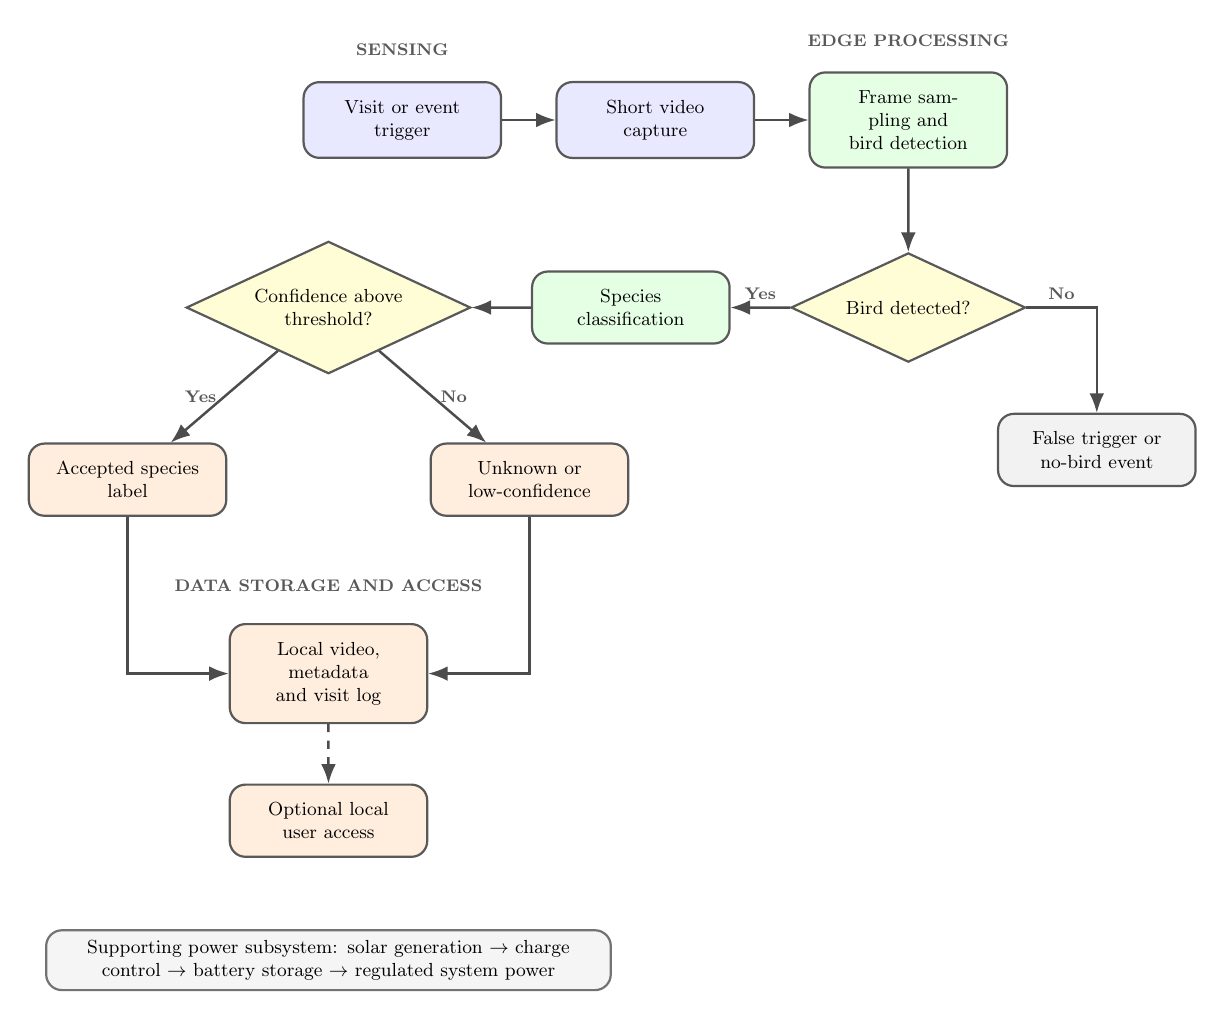
\begin{tikzpicture}[
        scale=0.76,
        transform shape,
        font=\small,
        >=Latex,
        line/.style={draw=black!70,line width=0.9pt,-{Latex[length=2.5mm]}},
        optional/.style={line,dashed},
        process/.style={
            rectangle,
            rounded corners=2mm,
            draw=black!65,
            line width=0.8pt,
            align=center,
            minimum height=11mm,
            text width=27mm,
            inner sep=3mm
        },
        sensing/.style={process,fill=blue!9},
        processing/.style={process,fill=green!10},
        output/.style={process,fill=orange!13},
        neutral/.style={process,fill=black!5},
        decision/.style={
            diamond,
            aspect=2.15,
            draw=black!65,
            line width=0.8pt,
            fill=yellow!16,
            align=center,
            text width=25mm,
            inner sep=1.5mm
        },
        power/.style={
            rectangle,
            rounded corners=2mm,
            draw=black!55,
            line width=0.8pt,
            fill=black!4,
            align=center,
            minimum height=10mm,
            text width=92mm
        },
        stage/.style={
            font=\footnotesize\bfseries,
            text=black!65
        }
    ]

        % Sensing and capture
        \node[sensing] (trigger)
            {Visit or event\\trigger};

        \node[sensing, right=9mm of trigger] (capture)
            {Short video\\capture};

        \node[processing, right=9mm of capture] (detect)
            {Frame sampling and\\bird detection};

        % Detection and classification
        \node[decision, below=14mm of detect] (bird)
            {Bird detected?};

        \node[processing, left=10mm of bird] (classify)
            {Species\\classification};

        \node[decision, left=10mm of classify] (confidence)
            {Confidence above\\threshold?};

        % Processing outcomes
        \node[neutral, below right=13mm and 5mm of bird] (false)
            {False trigger or\\no-bird event};

        \node[output, below left=17mm and 5mm of confidence] (accepted)
            {Accepted species\\label};

        \node[output, below right=17mm and 5mm of confidence] (unknown)
            {Unknown or\\low-confidence};

        \node[output, below=24mm of $(accepted)!0.5!(unknown)$] (storage)
            {Local video, metadata\\and visit log};

        \node[output, below=10mm of storage] (access)
            {Optional local\\user access};

        % Main information flow
        \draw[line] (trigger) -- (capture);
        \draw[line] (capture) -- (detect);
        \draw[line] (detect) -- (bird);

        \draw[line]
            (bird) --
            node[above,stage] {Yes}
            (classify);

        \draw[line] (classify) -- (confidence);

        \draw[line]
            (bird) -|
            node[above,stage,near start] {No}
            (false);

        \draw[line]
            (confidence) --
            node[left,stage] {Yes}
            (accepted);

        \draw[line]
            (confidence) --
            node[right,stage] {No}
            (unknown);

        \draw[line] (accepted) |- (storage);
        \draw[line] (unknown) |- (storage);
        \draw[optional] (storage) -- (access);

        % Power subsystem
        \node[power, below=12mm of access] (powersystem)
            {Supporting power subsystem:
             solar generation $\rightarrow$ charge control
             $\rightarrow$ battery storage
             $\rightarrow$ regulated system power};

        % Stage labels
        \node[stage, above=3mm of trigger]
            {SENSING};

        \node[stage, above=3mm of detect]
            {EDGE PROCESSING};

        \node[stage, above=4mm of storage]
            {DATA STORAGE AND ACCESS};

    \end{tikzpicture}

    \caption{Generic functional pipeline for an autonomous, camera-based bird-monitoring system. Solid arrows represent the primary data path, while the dashed arrow represents optional user access.}

    \label{fig:generic-monitoring-pipeline}
\end{figure}

\subsection{Camera-based monitoring}

%\begin{itemize}
%    \item \sout{Still images versus video.}
%    \item \sout{Continuous versus event-triggered recording.} 
%    \item \sout{Benefits and limitations of video for recording visits.}
%\end{itemize}

Although acoustic recording is regarded as a reliable means of remote bird monitoring, this project will instead use a camera-based system. As most existing smart bird feeders similarly use this medium, its benefits and drawbacks should be investigated.
\par\vspace{6pt}
As this project aims to provide non-invasive species identification using computer vision and ML, an important design decision is whether to record video or still images. Still images require significantly less storage and power \cite{GreenEtAl2023,JanischEtAl2021}, while video provides a richer user experience and is associated with improved species-identification accuracy \cite{GreenEtAl2023}.
\par\vspace{6pt}
Video recording is less efficient in terms of both energy and storage, influencing whether the system should monitor continuously or use a trigger mechanism. Given the project's dependence on solar power, continuous camera monitoring would impose excessive energy requirements, so a triggered system will be implemented \cite{JanischEtAl2021}. Although triggering significantly reduces power consumption, it introduces reliability concerns, including false triggers of an empty feeder and missed visits. Calibration and field testing must therefore be prioritised to minimise these events \cite{NeweyEtAl2015}. 
\par\vspace{6pt}
Having reviewed some of the means of monitoring bird remotely, a comparison of them can be conducted and their trade-offs evaluated. The principal trade-offs associated with media format and capture activation are summarised in Table~\ref{tab:capture-strategy-tradeoffs}.
\clearpage

\begin{table}[htbp]
    \centering
    \caption{Trade-offs between alternative media formats and capture strategies for autonomous bird monitoring.}
    \label{tab:capture-strategy-tradeoffs}

    \footnotesize
    \setlength{\tabcolsep}{4.5pt}
    \renewcommand{\arraystretch}{1.22}

    \begin{tabularx}{\textwidth}{
        >{\raggedright\arraybackslash}p{0.14\textwidth}
        >{\raggedright\arraybackslash}X
        >{\raggedright\arraybackslash}X
        >{\raggedright\arraybackslash}p{0.22\textwidth}
    }
        \toprule
        \textbf{Option}
        & \textbf{Principal advantages}
        & \textbf{Principal limitations}
        & \textbf{Suitability for this project} \\
        \midrule

        \multicolumn{4}{l}{
            \textbf{\textit{Media format}}
        } \\
        \addlinespace[2pt]

        Still images
        & Require relatively little storage and processing; individual images can be captured and classified quickly; impose a lower power demand than video.
        & Provide only one viewpoint per capture; may contain motion blur, occlusion or an unsuitable pose; cannot directly record visit duration or movement.
        & Moderate. Suitable for basic identification, but a single image may not provide sufficient evidence for reliable classification. \\

        \addlinespace

        Short video clips
        & Provide multiple frames and viewpoints; support selection of the clearest frame; record visit duration and offer a more complete visual record.
        & Require more storage, processing time and energy than still images; may produce redundant or unusable frames.
        & \textbf{High.} The additional visual information improves the likelihood of recording a useful view while keeping resource use manageable. \\

        \midrule

        \multicolumn{4}{l}{
            \textbf{\textit{Capture activation}}
        } \\
        \addlinespace[2pt]

        Continuous capture
        & Minimises dependence on trigger performance; provides complete coverage of activity within the camera field of view.
        & Produces large volumes of irrelevant footage; imposes high storage, processing and power demands; reduces battery-supported operating time.
        & Low. The resource demand conflicts with the requirements for portable, solar-powered operation. \\

        \addlinespace

        Event-triggered capture
        & Records media only when activity is detected; substantially reduces unnecessary storage, processing and energy use.
        & Performance depends on trigger sensitivity and positioning; delayed, missed or false activations may occur and must be evaluated experimentally.
        & \textbf{High.} It provides the most practical balance between visit coverage and resource consumption for autonomous deployment. \\

        \bottomrule
    \end{tabularx}

    \vspace{0.5em}

    \begin{minipage}{0.96\textwidth}
        \footnotesize
        \textit{Design implication:} Short, event-triggered video clips provide
        the most suitable combined strategy for the proposed system. This
        approach retains the principal identification benefits of video while
        limiting the storage and energy demands associated with continuous
        recording.
    \end{minipage}
\end{table}

\subsection{Automated species detection}

%\begin{itemize}
%    \item \sout{General development of image-based bird classification.} 
%    \item \sout{Challenges of fine-grained species recognition.} 
%    \item \sout{Curated datasets versus real field performance.} 
%    \item \sout{Benefits of a small, locally relevant class set.}
%    \item \sout{Need for low-confidence or unknown predictions.}
%\end{itemize}

Although rapid advances in ML and computer vision have made automated species identification increasingly feasible, several implementation decisions remain.
\par\vspace{6pt}
Such algorithms can achieve accuracies comparable to humans when implemented correctly, with researchers reporting 99.3\% accuracy for mammal identification \cite{NorouzzadehEtAl2018}. Similar results have been obtained for birds, with one study reporting 96.71\% accuracy across 10 species \cite{ChalmersEtAl2023}.
\par\vspace{6pt}
Bird identification using computer vision relies on fine-grained image classification (FGIC). Unlike conventional image classification, which distinguishes between distinct categories such as a ball and a dog, FGIC distinguishes between visually similar subcategories, such as dog breeds \cite{GeeksforGeeks2025FGIC}. FGIC is particularly sensitive to insufficient training data, but institutions and crowd-sourced initiatives have made large labelled datasets such as ImageNet and NABirds publicly available \cite{VanHornEtAl2015}.
\par\vspace{6pt}
Despite high benchmark accuracies, model performance can deteriorate substantially when algorithms trained on idealised online datasets are deployed in the field. Error rates have been found to increase by 92\% to 115\% under field conditions \cite{BeeryEtAl2018}. This highlights the importance of incorporating geographically relevant training data.
\par\vspace{6pt}
Public bird datasets can be extensive. Birds 525 contains nearly 90 thousand labelled images across 525 species \cite{PiosenkaBirds525}, while Semi-Aves contains over 160 thousand images across 1 000 species \cite{SuMaji2021}. The image and class scales of several commonly used bird-identification datasets are compared in Figure~\ref{fig:bird-dataset-scale}. However, narrowing the training scope can improve performance. One study found that removing the rarest species increased identification accuracy from 72.8\% to 76.3\% \cite{NormanEtAl2023}. Using a smaller, locally relevant class set is also common in automated bird-identification studies \cite{Mansouri2025, NormanEtAl2023}. The model used in this project will therefore be limited to bird species relevant to Cape Town. 
\par\vspace{6pt}

\begin{figure}[htbp]
    \centering

    % Image-count chart
    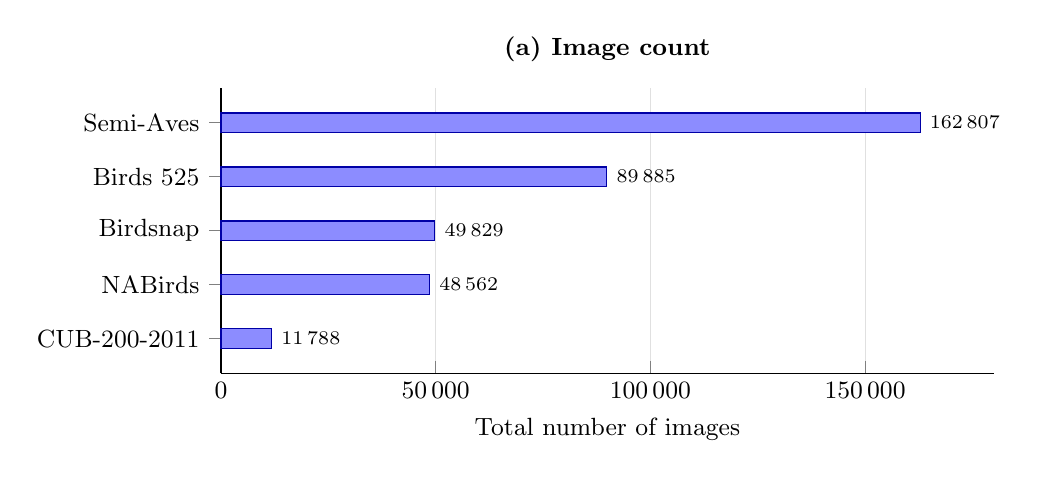
\begin{tikzpicture}
        \begin{axis}[
            width=0.94\textwidth,
            height=5.2cm,
            xbar,
            bar width=7pt,
            xmin=0,
            xmax=180000,
            xtick={0,50000,100000,150000},
            scaled x ticks=false,
            xticklabel style={
                /pgf/number format/fixed,
                /pgf/number format/1000 sep={\,}
            },
            xlabel={Total number of images},
            ytick={1,2,3,4,5},
            yticklabels={
                CUB-200-2011,
                NABirds,
                Birdsnap,
                Birds 525,
                Semi-Aves
            },
            yticklabel style={font=\small},
            tick label style={font=\small},
            label style={font=\small},
            axis x line*=bottom,
            axis y line*=left,
            xmajorgrids=true,
            grid style={draw=black!12},
            enlarge y limits=0.16,
            nodes near coords={
                \pgfmathprintnumber[
                    fixed,
                    precision=0,
                    1000 sep={\,}
                ]{\pgfplotspointmeta}
            },
            nodes near coords align={horizontal},
            every node near coord/.append style={
                font=\scriptsize,
                anchor=west
            },
            point meta=x,
            clip=false,
            title={(a) Image count},
            title style={font=\small\bfseries}
        ]
            \addplot[
                draw=blue!65!black,
                fill=blue!45
            ] coordinates {
                (11788,1)
                (48562,2)
                (49829,3)
                (89885,4)
                (162807,5)
            };
        \end{axis}
    \end{tikzpicture}

    \vspace{0.5em}

    % Class-count chart
    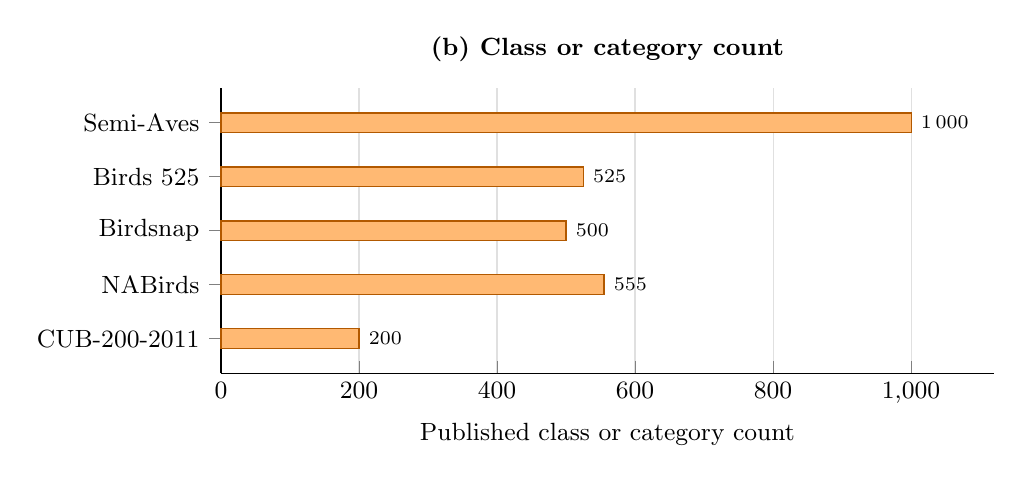
\begin{tikzpicture}
        \begin{axis}[
            width=0.94\textwidth,
            height=5.2cm,
            xbar,
            bar width=7pt,
            xmin=0,
            xmax=1120,
            xtick={0,200,400,600,800,1000},
            scaled x ticks=false,
            xlabel={Published class or category count},
            ytick={1,2,3,4,5},
            yticklabels={
                CUB-200-2011,
                NABirds,
                Birdsnap,
                Birds 525,
                Semi-Aves
            },
            yticklabel style={font=\small},
            tick label style={font=\small},
            label style={font=\small},
            axis x line*=bottom,
            axis y line*=left,
            xmajorgrids=true,
            grid style={draw=black!12},
            enlarge y limits=0.16,
            nodes near coords={
                \pgfmathprintnumber[
                    fixed,
                    precision=0,
                    1000 sep={\,}
                ]{\pgfplotspointmeta}
            },
            nodes near coords align={horizontal},
            every node near coord/.append style={
                font=\scriptsize,
                anchor=west
            },
            point meta=x,
            clip=false,
            title={(b) Class or category count},
            title style={font=\small\bfseries}
        ]
            \addplot[
                draw=orange!70!black,
                fill=orange!55
            ] coordinates {
                (200,1)
                (555,2)
                (500,3)
                (525,4)
                (1000,5)
            };
        \end{axis}
    \end{tikzpicture}

    \caption[
        Comparison of the scale of selected bird-image datasets
    ]{
        Scale of selected bird-image datasets by total image count
        and published class or category count. Adapted from dataset
        statistics reported by Wah et al. \cite{WahEtAl2011},
        Van Horn et al. \cite{VanHornEtAl2015},
        Berg et al. \cite{BergEtAl2014},
        Gpiosenka \cite{Birds525Dataset}, and
        Su and Maji \cite{SuMaji2021}.
    }
    \label{fig:bird-dataset-scale}

    \vspace{0.4em}
\end{figure}

A smaller class set introduces the challenge of handling unidentified birds and other off-target detections. Two scenarios must be considered: low-confidence predictions and classes unknown to the model. Low-confidence predictions can be handled using selective classification, or a "reject option", in which predictions below a confidence threshold are rejected \cite{GeifmanElYaniv2017}. Unknown classes arise because the model operates in an open-set environment, where it may encounter classes absent from its training data \cite{ScheirerEtAl2013}. A similar rejection mechanism should therefore be used to prevent unreliable classification of unknown visitors.


\subsection{Embedded and autonomous usage}

%\begin{itemize}
%    \item \sout{Advantages of edge processing.}
%    \item \sout{General computational and energy constraints.}
%    \item \sout{Solar-powered wildlife-monitoring systems.}
%\end{itemize}

Given that this project aims to rely on solar power for continuous remote operation, literature concerning its embedded and autonomous functionality must also be reviewed.
\par\vspace{6pt}
While most existing smart feeders discussed previously rely on external servers or cloud services for data storage and processing, this project will instead perform these functions on-device using edge processing. Besides removing dependence on remote processing, edge processing enables immediate decisions on whether footage should be recorded, reducing storage of irrelevant data \cite{DarrasEtAl2024}.
\par\vspace{6pt}
This project requires an inference model capable of identifying bird visits quickly enough to determine whether recording should occur. Microcontrollers offer low-power operation and are well suited to simple sensing and processing, but their limited architecture restricts demanding tasks such as inference and image classification. Consequently, these tasks generally take considerably longer than on a microcomputer, limiting the suitability of microcontrollers for neural-network applications \cite{BallerEtAl2021}.
\par\vspace{6pt}
Microcomputers provide greater processing capability but require significantly more power while operating. Trigger-based recording can reduce storage requirements, but will only similarly reduce power consumption if components, or the system as a whole, can enter and exit an idle state when inactive \cite{BalleEtAl2025}. The principal differences between conventional microcontrollers and Raspberry Pi--class single-board computers are summarised in Table~\ref{tab:microcontroller-sbc-comparison}.

\par\vspace{6pt}

\begin{table}[htbp]
    \centering
    \caption{Comparison of conventional microcontrollers and Raspberry Pi--class single-board computers.}
    \label{tab:microcontroller-sbc-comparison}

    \footnotesize
    \setlength{\tabcolsep}{4pt}
    \renewcommand{\arraystretch}{1.2}

    \begin{tabularx}{\textwidth}{
        >{\raggedright\arraybackslash}p{0.13\textwidth}
        >{\raggedright\arraybackslash}X
        >{\raggedright\arraybackslash}X
        >{\raggedright\arraybackslash}p{0.22\textwidth}
    }
        \toprule
        \textbf{Criterion}
        & \textbf{Microcontroller}
        & \textbf{Raspberry Pi--class SBC}
        & \textbf{Project relevance} \\
        \midrule

        Power
        & Very low consumption with effective sleep modes.
        & Typically consumes several watts when active.
        & Microcontrollers offer better low-power operation. \\

        \addlinespace

        Start-up
        & Begins operating almost immediately.
        & Requires several seconds to boot.
        & Frequent SBC power cycling may delay capture. \\

        \addlinespace

        Memory
        & Usually kilobytes to a few megabytes.
        & Commonly provides several gigabytes.
        & Video processing requires SBC-level memory. \\

        \addlinespace

        Camera and video
        & Limited resolution and video-handling capability.
        & Supports high-resolution cameras and sustained video capture.
        & Short-video recording favours the SBC. \\

        \addlinespace

        Machine learning
        & Restricted mainly to compact TinyML models.
        & Supports larger models and inference accelerators.
        & Species classification favours the SBC. \\

        \addlinespace

        Software
        & Runs embedded firmware or a real-time operating system.
        & Runs Linux with established camera and ML libraries.
        & The SBC simplifies system integration. \\

        \addlinespace

        Data and web access
        & Storage, databases and web services are constrained.
        & Supports local storage, databases and web servers.
        & Required for visit logging and the web interface. \\

        \addlinespace

        Reliability
        & Simple software stack and rapid recovery.
        & Requires storage, thermal and shutdown management.
        & SBC reliability must be addressed in the design. \\

        \midrule

        Recommended role
        & Optional trigger or power-management controller.
        & \textbf{Primary system processor.}
        & Add a microcontroller only if testing demonstrates a need. \\

        \bottomrule
    \end{tabularx}

    \vspace{0.4em}
\end{table}

For a system to operate continuously using only solar power, the usable solar energy generated must meet or exceed the system's energy demand and associated losses:

$$
E_{\text{solar, usable}} \geq E_{\text{system}} + E_{\text{losses}}
$$

\par\vspace{6pt}
Although most smart feeders reviewed previously rely on external power, commercial products such as the Birdfy and academic studies demonstrate that solar-powered operation is feasible \cite{BirdfyHumFeeder,PouRossellEtAl2025}.
\par\vspace{6pt}
Having investigated the key technologies supporting the proposed system, a clearer basis for the design phase has been established. The advantages and limitations of each technology have been considered to identify the options most suitable for this project.

\section{Conclusion}

With the relevant literature investigated, several conclusions can be drawn to support the motivation for this research and inform the design and methods of the proposed system.
\par\vspace{6pt}
Analysis of existing smart bird feeders provides insight into existing solutions and opportunities for improvement. Many systems use neural-network classification to automate non-invasive species identification. However, several rely on external processing, cloud services or network connectivity, limiting their suitability for remote deployment. Similarly, fully autonomous solar operation is not consistently demonstrated. These limitations support the use of local processing, storage and power generation in this project.
\par\vspace{6pt}
The review also identified relatively little research on smart nectar feeders, with most literature focused on seed feeders despite several commercial hummingbird feeders. Focusing on nectar-feeding birds introduces additional design considerations, including feeder colour, nectar replacement and protecting electronic components from nectar spillage and environmental exposure.
\par\vspace{6pt}
In conclusion, the literature reviewed proves the feasibility of the required technology for this project, but these proofs are hardly realised as a combined and complete smart nectar feeder for sunbirds. The findings from the literature support the use of triggered video capture, a locally relevant classification model, edge computing and local storage, together with autonomous solar power.
The basis for the system requirements and design decisions developed in the following chapters will be constructed using these findings.
\glsresetall % reset the glossary to expand acronyms again
\chapter{Methodology and Design}
\label{ch:Methodology}

\section{Introduction}
\label{sec:MethodologyIntro}

This chapter will be dedicated to describing the methodology used in designing and realising this project, as well as detailing the design choices and process. The first section of this chapter will deal with the former of these two topics. 
%\par\vspace{6pt}

\section{Project Methodology}
\label{sec:Methodology}

The goals and requirements of this project were stated in Chapter \ref{ch:Introduction} of this report. In Chapter \ref{ch:LitReview} I investigated the methods used by others to accomplish similar goals and meet similar requirements. Using this knowledge and input from my supervisor, I have devised an appropriate methodology to implement when undertaking this project. This methodology caters toward the specific nature of this project (many subsystems, hardware + software, etc), as well as the many constraints around this project (budget, time, etc).

Okay, so basically the method outline is:
\begin{enumerate}
    \item Identify problem
    \item Set goals and requirements
    \item Research literature and similar existing projects
    \item Decide overall system design
    \item Decide on what hardware and software to use
    \item Design and test each subsystem
    \item Assemble complete system and test
    \item Look for and make improvements where possible
    \item Cross-reference complete system against initial goals and requirements
    \item Measure and remark on results
    \item Identify future work and system's shortcomings, if applicable
    \item Prioritise something that works over something that would be cool if it worked
\end{enumerate}

\section{Requirements Definition}
\label{sec:RequirementsDefinition}

Again, the aims and goals of this project were stated in Chapter \ref{ch:Introduction}. As an engineer, it is important to translate these sometimes vague/broad points into technical requirements. Using the aims and goals in Chapter \ref{ch:Introduction} as an introduction, I developed the following requirements for the final system:
These requirements outline the appropriate final specifications needed for the system.

\subsection{Functional Requirements}
\label{subsec:FunctionalRequirements}
\begin{itemize}
    \item The system must detect any significant motion at the feeder port
    \item The system must trigger the classification algorithm once motion is detected
    \item The system must categorize detected subjects into a defined list of species
    \item The system must manage low-confidence or unrecognised classes appropriately
    \item The system must record a video if the classification algorithm determines the source of motion to be of a class of interest
    \item The system must store any recorded footage in a non-volatile storage medium
    \item The system must charge from a solar power source utilise a battery for energy storage
    \item The system must make recorded footage accessible from a self-hosted web page for users to interact with
    \item The system must utilize an 'energy-saving' mode when idle
    
\end{itemize}

\subsection{Non-Functional Requirements}
\label{subsec:NonFunctionalRequirements}
\begin{itemize}
    \item The system's feeder must be easily accessible and refillable
    \item The system must be able to classify within x seconds of motion detection
    \item Recording of a visit must begin y seconds after motion detection trigger
    \item Recorded footage should meet a minimum resolution/frame-rate requirement sufficient for classification
    \item Classification accuracy must be at least z\%
    \item False positive events must be less than a\%
    \item User interaction with the system's web interface must be intuitive, easy and well-documented
    \item The total Bill of Materials must amount to less than R\_
    \item The system must have an uptime of at least \_ hours per day, under full sunlight
    \item The electronic subsystem must be protected from environmental elements by the system's housing
    \item The system should not present sharp edges, trapping hazards or harmful contamination risks to birds
    \item Electronics must remain within their allowable operating temperature range during deployment
    \item The project must contain sufficient design and build documentation
\end{itemize}

\section{Acceptance Testing Procedures}
\label{sec:AcceptanceTestingProcedures}

Explain the experimental approach used to determine whether the completed system satisfied the requirements established in Section~\ref{sec:RequirementsDefinition}.
\par\vspace{6pt}
Main categories of system evaluation:
\begin{itemize}
    \item Mechanical and feeder performance: Verify feeder stability, enclosure protection, and ease of refilling and cleaning.
    
    \item Visit detection performance: Measure successful detections and false-positive and false-negative rates against the acceptance limits.
    
    \item Video capture performance: Verify that visits are sufficiently recorded and that image quality, focus, frame rate and camera positioning meet requirements.
    
    \item Data storage and logging: Verify that videos and metadata are stored correctly, retained after restart or power loss, and that storage remains reliable.
    
    \item Classification performance: Measure classification accuracy, false-identification rate, inference time, per-class performance where relevant, and low-confidence rejection performance.
    
    \item Web interface performance: Verify access to visit records, classification results and video playback, and confirm correct operation of required functions.
    
    \item Embedded-system performance and reliability: Run the system continuously for a defined period and record crashes, missed events, storage errors or interruptions. Verify automatic recovery where required.
    
    \item Power consumption and autonomy: Measure power use during idle, recording and classification, and determine battery runtime from a full charge.
    
    \item Solar charging performance: Measure whether the solar subsystem can recharge or sustain the battery under representative sunlight conditions.
    
    \item Overall integrated-system performance: Verify that visits are detected, recorded, classified, stored and made available to the user without manual intervention, and record any subsystem-integration failures.
\end{itemize}

\section{Design Decisions}
\label{sec:DesignDecisions}

Introduction to overall system, with basic block diagram of all the interacting subsystems. Explain the pipeline of operation briefly.

\begin{figure}[htbp]
\centering
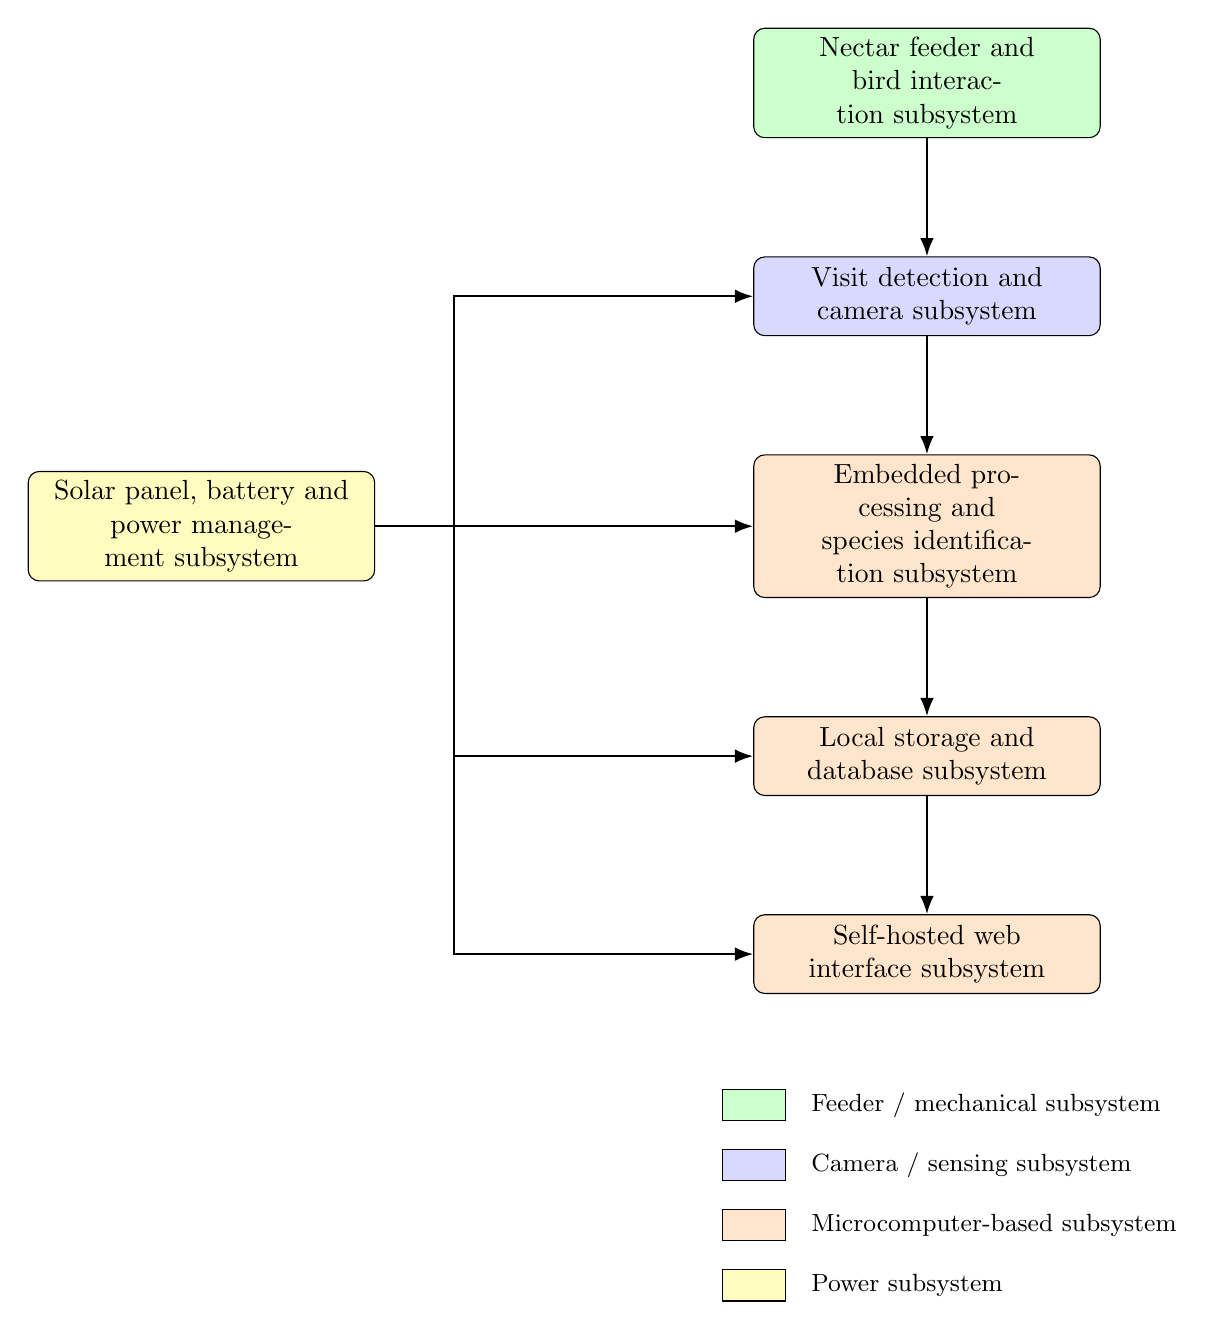
\begin{tikzpicture}[
    node distance=1.5cm and 1.8cm,
    >=Latex,
    block/.style={
        rectangle,
        draw,
        rounded corners,
        align=center,
        minimum width=4.4cm,
        minimum height=1.0cm,
        text width=4.0cm
    },
    feederblock/.style={
        block,
        fill=green!20
    },
    camerablock/.style={
        block,
        fill=blue!15
    },
    computerblock/.style={
        block,
        fill=orange!20
    },
    powerblock/.style={
        block,
        fill=yellow!25
    },
    line/.style={draw, -Latex, thick}
]

% Main blocks
\node[feederblock] (feeder) {Nectar feeder and\\bird interaction subsystem};

\node[camerablock, below=of feeder] (detection) {Visit detection and\\camera subsystem};

\node[computerblock, below=of detection] (processing) {Embedded processing and\\species identification subsystem};

\node[computerblock, below=of processing] (storage) {Local storage and\\database subsystem};

\node[computerblock, below=of storage] (web) {Self-hosted web\\interface subsystem};

\node[powerblock, left=4.8cm of processing] (power) {Solar panel, battery and\\power management subsystem};

% Main flow arrows
\draw[line] (feeder) -- (detection);
\draw[line] (detection) -- (processing);
\draw[line] (processing) -- (storage);
\draw[line] (storage) -- (web);

% Power connections
\draw[line] (power.east) -- ++(1.0,0) |- (detection.west);
\draw[line] (power.east) -- ++(1.0,0) |- (processing.west);
\draw[line] (power.east) -- ++(1.0,0) |- (storage.west);
\draw[line] (power.east) -- ++(1.0,0) |- (web.west);

% Colour legend
\node[
    rectangle,
    draw,
    fill=green!20,
    minimum width=0.8cm,
    minimum height=0.4cm,
    below=1.2cm of web,
    xshift=-2.2cm
] (leg1) {};

\node[
    anchor=west,
    right=0.2cm of leg1
] {\small Feeder / mechanical subsystem};


\node[
    rectangle,
    draw,
    fill=blue!15,
    minimum width=0.8cm,
    minimum height=0.4cm,
    below=0.35cm of leg1
] (leg2) {};

\node[
    anchor=west,
    right=0.2cm of leg2
] {\small Camera / sensing subsystem};


\node[
    rectangle,
    draw,
    fill=orange!20,
    minimum width=0.8cm,
    minimum height=0.4cm,
    below=0.35cm of leg2
] (leg3) {};

\node[
    anchor=west,
    right=0.2cm of leg3
] {\small Microcomputer-based subsystem};


\node[
    rectangle,
    draw,
    fill=yellow!25,
    minimum width=0.8cm,
    minimum height=0.4cm,
    below=0.35cm of leg3
] (leg4) {};

\node[
    anchor=west,
    right=0.2cm of leg4
] {\small Power subsystem};

\end{tikzpicture}
\caption{High-level block diagram of the proposed smart sunbird feeder system. Blocks are coloured according to the primary hardware subsystem on which they rely.}
\label{fig:system_block_diagram}
\end{figure}

\begin{figure}[htbp]
\centering
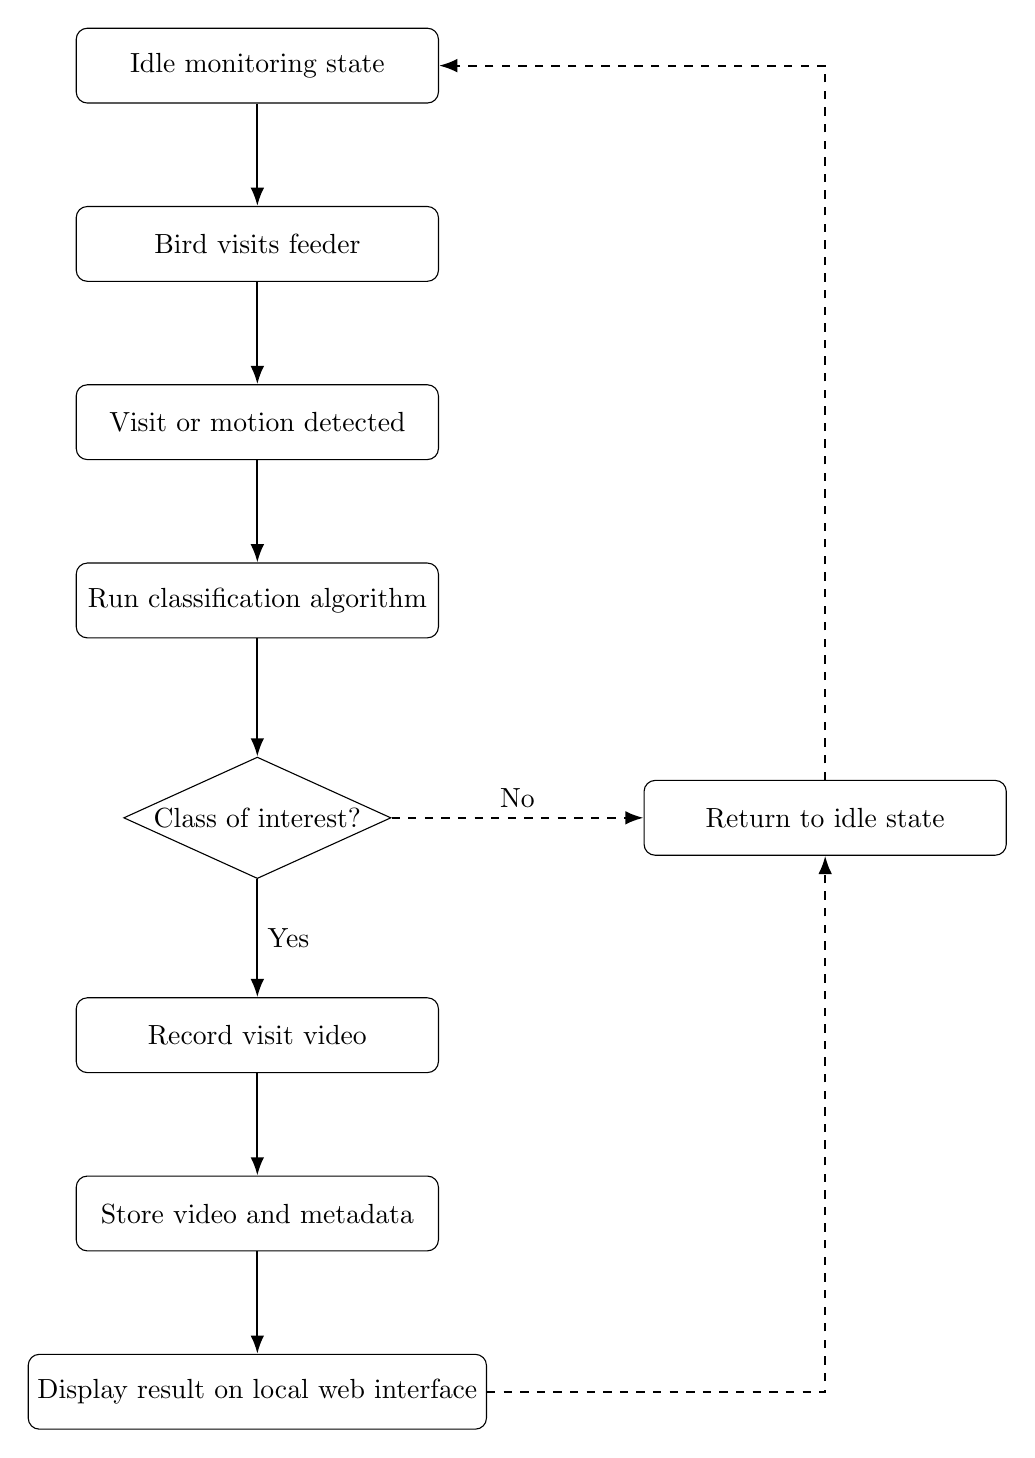
\begin{tikzpicture}[
    node distance=1.3cm,
    >=Latex,
    block/.style={
        rectangle,
        draw,
        rounded corners,
        align=center,
        minimum width=4.6cm,
        minimum height=0.95cm
    },
    decision/.style={
        diamond,
        draw,
        align=center,
        aspect=2.2,
        inner sep=1pt
    },
    line/.style={draw, -Latex, thick},
    dashedline/.style={draw, -Latex, dashed, thick}
]

\node[block] (idle) {Idle monitoring state};
\node[block, below=of idle] (visit) {Bird visits feeder};
\node[block, below=of visit] (detect) {Visit or motion detected};
\node[block, below=of detect] (classify) {Run classification algorithm};
\node[decision, below=1.5cm of classify] (decision) {Class of interest?};
\node[block, below=1.5cm of decision] (record) {Record visit video};
\node[block, below=of record] (store) {Store video and metadata};
\node[block, below=of store] (display) {Display result on local web interface};

\node[block, right=3.2cm of decision] (returnidle) {Return to idle state};

\draw[line] (idle) -- (visit);
\draw[line] (visit) -- (detect);
\draw[line] (detect) -- (classify);
\draw[line] (classify) -- (decision);
\draw[line] (decision) -- node[right] {Yes} (record);
\draw[line] (record) -- (store);
\draw[line] (store) -- (display);
\draw[dashedline] (decision.east) -- node[above] {No} (returnidle.west);
\draw[dashedline] (display.east) -| (returnidle.south);
\draw[dashedline] (returnidle.north) |- (idle.east);

\end{tikzpicture}
\caption{Operational pipeline of the proposed smart sunbird feeder system.}
\label{fig:system_pipeline}
\end{figure}

\subsection{Hardware Design Decisions}
\label{subsec:HardwareDesignDecisions}

\paragraph{Microcomputer}

Reiterate that a microcontroller is inadequate for the inference speed required for this project. Basically, besides the fact that we already had it, the RPi 4B was chosen because:

\begin{itemize}
    \item It is the least computationally-expensive option that can get the job done
    \item It is also one of the more budget-friendly options that can get the job done
    \item Unlike its more expensive couterparts, the 4B has onboard FHD video encoding, which is much less power intensive when recording and storing videos
    \item It was already available and has been proven to work well for a similar application, so less design risk and lead time
\end{itemize}

The candidate platforms were compared according to processing capability, camera compatibility, software support, energy consumption and integration risk. Table~\ref{tab:microcomputer-comparison} shows that the Raspberry Pi 4B provides the most appropriate balance for the project.

\begin{table}[htbp]
    \centering
    \caption{Comparison of candidate processing platforms}
    \label{tab:microcomputer-comparison}
    \small
    \renewcommand{\arraystretch}{1.15}

    \begin{tabularx}{\textwidth}{
        >{\raggedright\arraybackslash}p{2.2cm}
        >{\raggedright\arraybackslash}X
        >{\centering\arraybackslash}p{1.3cm}
        >{\centering\arraybackslash}p{1.9cm}
        >{\raggedright\arraybackslash}X}

        \toprule
        \textbf{Platform} & \textbf{Key capability} &
        \textbf{Power} & \textbf{Approx. cost} &
        \textbf{Assessment} \\
        \midrule

        \rowcolor{green!12}
        \textbf{Raspberry Pi 4B} &
        Native Camera Module 3 support and sufficient ML performance &
        Moderate &
        R0\textsuperscript{*} &
        \textbf{Selected:} sufficient performance, lower energy demand and no acquisition cost. \\

        Raspberry Pi 5 4GB &
        Faster CPU and greater processing headroom &
        High &
        R2\,845 \cite{CommunicaRPi5} &
        Extra performance did not justify its higher cost and power demand. \\

        NVIDIA Jetson Orin Nano Super &
        GPU acceleration providing up to 67 TOPS &
        Very high &
        R8\,669 \cite{RSJetsonOrinNano} &
        Powerful, but well above the budget and unsuitable for solar operation. \\

        ESP32-S3 &
        Low-power microcontroller with wireless connectivity &
        Very low &
        R200 \cite{PiShopESP32S3} &
        Unable to support the required camera, video and Linux-based ML stack. \\

        \bottomrule
    \end{tabularx}

    \vspace{2pt}
    \footnotesize{\textsuperscript{*}The Raspberry Pi 4B was supplied at no
    project cost. A comparable 4GB board retailed for approximately
    R1\,639 \cite{PrototypeDIYRPi4B}. Prices include VAT and were accessed
    on 16 September 2026.}
\end{table}

\paragraph{Camera Module}
\par\vspace{6pt}
Introduce the Camera Module 3 as the standard camera module for RPis. Mention the other types of camera modules and then explain why the basic Camera Module 3 was eventually chosen:
\begin{itemize}
    \item It has ample resolution and framerate for the task at hand
    \item It doesn't have an IR filter, which helps identify the iridescent sunbirds much more easily
    \item It is the most affordable camera module in the family
    \item It has a variable focus, which the cheaper Module 2 does not
\end{itemize}
Talk about how the more expensive modules were unnecessarily complicating the objective at a higher price
The candidate cameras were compared according to image quality, focusing capability, cost and integration requirements, as summarised in Table~\ref{tab:camera-comparison}.
\begin{table}[htbp]
    \centering
    \caption{Comparison of candidate camera modules}
    \label{tab:camera-comparison}
    \small
    \renewcommand{\arraystretch}{1.15}
    
    \begin{tabularx}{\textwidth}{
        >{\raggedright\arraybackslash}p{2.4cm}
        >{\raggedright\arraybackslash}p{2.3cm}
        >{\centering\arraybackslash}p{1.6cm}
        >{\centering\arraybackslash}p{2.2cm}
        >{\raggedright\arraybackslash}X}
        
        \toprule
        \textbf{Camera} & \textbf{Imaging capability} &
        \textbf{Focus} & \textbf{Approx. cost} &
        \textbf{Assessment} \\
        \midrule
        
        \rowcolor{green!12}
        \textbf{Camera Module 3} &
        12\,MP, HDR &
        Autofocus &
        R0\textsuperscript{*} &
        \textbf{Selected:} best balance of image quality, size, compatibility and cost. \\
        
        Camera Module 2 &
        8\,MP &
        Fixed &
        R290 \cite{PrototypeDIYCameraModule2} &
        Lower resolution and limited focusing flexibility. \\
        
        HQ Camera and lens &
        12.3\,MP, adjustable optics &
        Manual &
        R1\,950 \cite{PiShopHQCamera,PiShopZoomLens} &
        Greater optical control, but bulky and unnecessarily expensive. \\
        
        Raspberry Pi AI Camera &
        12\,MP, on-sensor inference &
        Manual &
        R1\,325 \cite{PiShopAICamera} &
        Onboard inference adds cost and deployment complexity. \\
        
        \bottomrule
    \end{tabularx}
    
    \vspace{2pt}
    \footnotesize{\textsuperscript{*}The Camera Module 3 was provided at no cost; its retail price was approximately R505 \cite{PiShopCameraModule3}. Prices include VAT.}
\end{table}

\paragraph{Motion Sensor}
\par\vspace{6pt}
Introduce the VL53L1X ToF sensor as the chosen motion sensor and justify its use over others because:
\begin{itemize}
    \item Programmable FOV, which decreases risk of background distrubances triggering it
    \item Interrupt output for RPi triggering without camera monitoring
    \item 50Hz measurement rate. Very fast response time
    \item ToF sensors enable birds to remain detected while stationary and feeding
    \item Its infrared emitter is eye-safe
    \item Ideal for short-range detection, with an adjustable threshold
\end{itemize}

Candidate visit-detection sensors were compared according to their detection method, sensing region, cost and suitability for monitoring the feeder port, as shown in Table~\ref{tab:motion-sensor-comparison}.

\begin{table}[htbp]
    \centering
    \caption{Comparison of candidate visit-detection sensors}
    \label{tab:motion-sensor-comparison}
    \small
    \renewcommand{\arraystretch}{1.15}
    
    \begin{tabularx}{\textwidth}{
        >{\raggedright\arraybackslash}p{2.2cm}
        >{\raggedright\arraybackslash}p{2.2cm}
        >{\centering\arraybackslash}p{2.0cm}
        >{\centering\arraybackslash}p{1.8cm}
        >{\raggedright\arraybackslash}X}
        
        \toprule
        \textbf{Sensor} & \textbf{Detection method} &
        \textbf{Detection region} & \textbf{Approx. cost} &
        \textbf{Assessment} \\
        \midrule
        
        \rowcolor{green!12}
        \textbf{VL53L1X} &
        Optical time-of-flight &
        Up to 4\,m; adjustable region &
        R220 \cite{MantechVL53L1X} &
        \textbf{Selected:} precise detection zone and reliable stationary-object detection. \\
        
        HC-SR501 &
        Passive infrared &
        Wide, adjustable cone &
        R22 \cite{PiShopHCSR501} &
        Low power, but detects thermal motion rather than feeder occupancy. \\
        
        HC-SR04 &
        Ultrasonic ranging &
        0.02--4\,m cone &
        R37 \cite{DIYEHCSR04} &
        Low cost, but less directional and sensitive to outdoor conditions. \\
        
        VL53L0X &
        Optical time-of-flight &
        Up to 2\,m; fixed region &
        R40 \cite{PiShopVL53L0X} &
        Cheaper, but offers less range and detection-region control. \\
        
        \bottomrule
    \end{tabularx}
\end{table}

\paragraph{Solar Power System}
\par\vspace{6pt}
Waveshare Model B power management system with MP 133x110 2.4W panel
\begin{itemize}
    \item Wide input range of solar voltage: 6-24V
    \item Protection against overcharging, over-discharging, excessive current, overheating and reversed solar-panel polarity
    \item USB-C charging capability in case of insufficient solar energy input
    \item 5V/3A output matches RPi power input requirements
\end{itemize}

\paragraph{Housing}
\par\vspace{6pt}
3D printed with white PLA because:
\begin{itemize}
    \item Cheap and easily accessible thanks to the university's printing lab.
    \item Ideal for frequently-evolving prototypes that require quick production.
    \item Allows for an entirely customisable shape and features as required by the project.
    \item White colour specifically to minimise the heat absorbed from the sun and helps keep electronics cool.
\end{itemize}

\subsection{Software Design Decisions}
\label{subsec:SoftwareDesignDecisions}

\paragraph{Operating System}
\par\vspace{6pt}
Introduce RPi Lite x64 as the selected OS, among several candidate OSs for the RPi 4B. It was selected because:
\begin{itemize}
    \item It is headless, which meant it is one of the least computationally and energy-intensive OSs since there are no unneeded applications etc running
    \item It is 64-bit, which makes it compatible for use with all the libraries used by the classification algorithm. 32-bit would not have worked
\end{itemize}

The correct term is Raspberry Pi OS Lite (64-bit/ARM64) rather than x64, which normally refers to the x86-64 architecture. The candidates were compared according to resource demand, hardware support and software compatibility, as summarised in Table~\ref{tab:os-comparison}.

\begin{table}[htbp]
    \centering
    \caption{Comparison of candidate operating systems}
    \label{tab:os-comparison}
    \small
    \renewcommand{\arraystretch}{1.15}

    \begin{tabularx}{\textwidth}{
        >{\raggedright\arraybackslash}p{2.7cm}
        >{\centering\arraybackslash}p{1.5cm}
        >{\centering\arraybackslash}p{1.5cm}
        >{\raggedright\arraybackslash}X
        >{\raggedright\arraybackslash}X}

        \toprule
        \textbf{Operating system} & \textbf{Interface} &
        \textbf{Demand} & \textbf{Project compatibility} &
        \textbf{Assessment} \\
        \midrule

        \rowcolor{green!12}
        \textbf{Raspberry Pi OS Lite 64-bit}
        \cite{RaspberryPiOS,RaspberryPiOS64} &
        Headless &
        Low &
        Native camera and GPIO support; compatible with ARM64 ML software &
        \textbf{Selected:} provides the required functionality with minimal overhead. \\

        Raspberry Pi OS Lite 32-bit
        \cite{RaspberryPiOS} &
        Headless &
        Low &
        Native hardware support, but limited to ARM32 software &
        Suitable for legacy software, but offers less ML compatibility and performance headroom. \\

        Raspberry Pi OS Desktop 64-bit
        \cite{RaspberryPiOS} &
        Desktop GUI &
        Higher &
        Same Raspberry Pi hardware support &
        The graphical desktop unnecessarily consumes storage, memory and processing resources. \\

        Ubuntu Server 64-bit
        \cite{UbuntuRaspberryPi} &
        Headless &
        Moderate &
        Supports the Pi 4B, but requires more Pi-specific configuration &
        Capable, but less directly aligned with the official camera software stack. \\

        \bottomrule
    \end{tabularx}
\end{table}

\paragraph{Classification Model}
\par\vspace{6pt}
EfficientNetV2 was chosen as the convolutional backbone of the classification model, pretrained on the ImageNet dataset.

\paragraph{Dataset}
\par\vspace{6pt}
Mention licensing and their corresponding usage limitations.

\paragraph{Web Page}
\par\vspace{6pt}


\section{Conclusion}
\label{sec:MethodologyConclusion}


% Chapter 4 - Design

\glsresetall % reset the glossary to expand acronyms again
\chapter[Design]{Design}\label{ch:Design}
\index{Design}

\section{Introduction}
\label{sec:DesignIntroduction}

The purpose of this chapter will be to present, in detail, the design of a smart sunbird feeder. The design explained in this chapter will build on the information presented in the previous chapters. The design approach used for this system follows the methodology and design decisions established in Chapter~\ref{ch:Methodology}. As this system comprises of several hardware and software subsystems, this chapter will describe each subsystem in its own subsection. 

\section{Hardware Design}
\label{sec:HardwareDesign}

This section details the design of the physical/material subsystems and components of which the system is comprised. Overall, the subsystems comprising of the system's hardware are connected to each other through electrical and communication interfaces. The interaction between all of the hardware subsystems is represented in Figure~\ref{fig:hardware_block_diagram}, which shows the power and signal connections between each of the components. The hardware design of the system is presented in the following subsections, which include the feeder and mechanical design, embedded computing and camera, visit-detection hardware, storage and hardware interfaces, power and solar system, and enclosure and outdoor installation.

\begin{figure}[htbp]
\centering
\resizebox{\textwidth}{!}{%
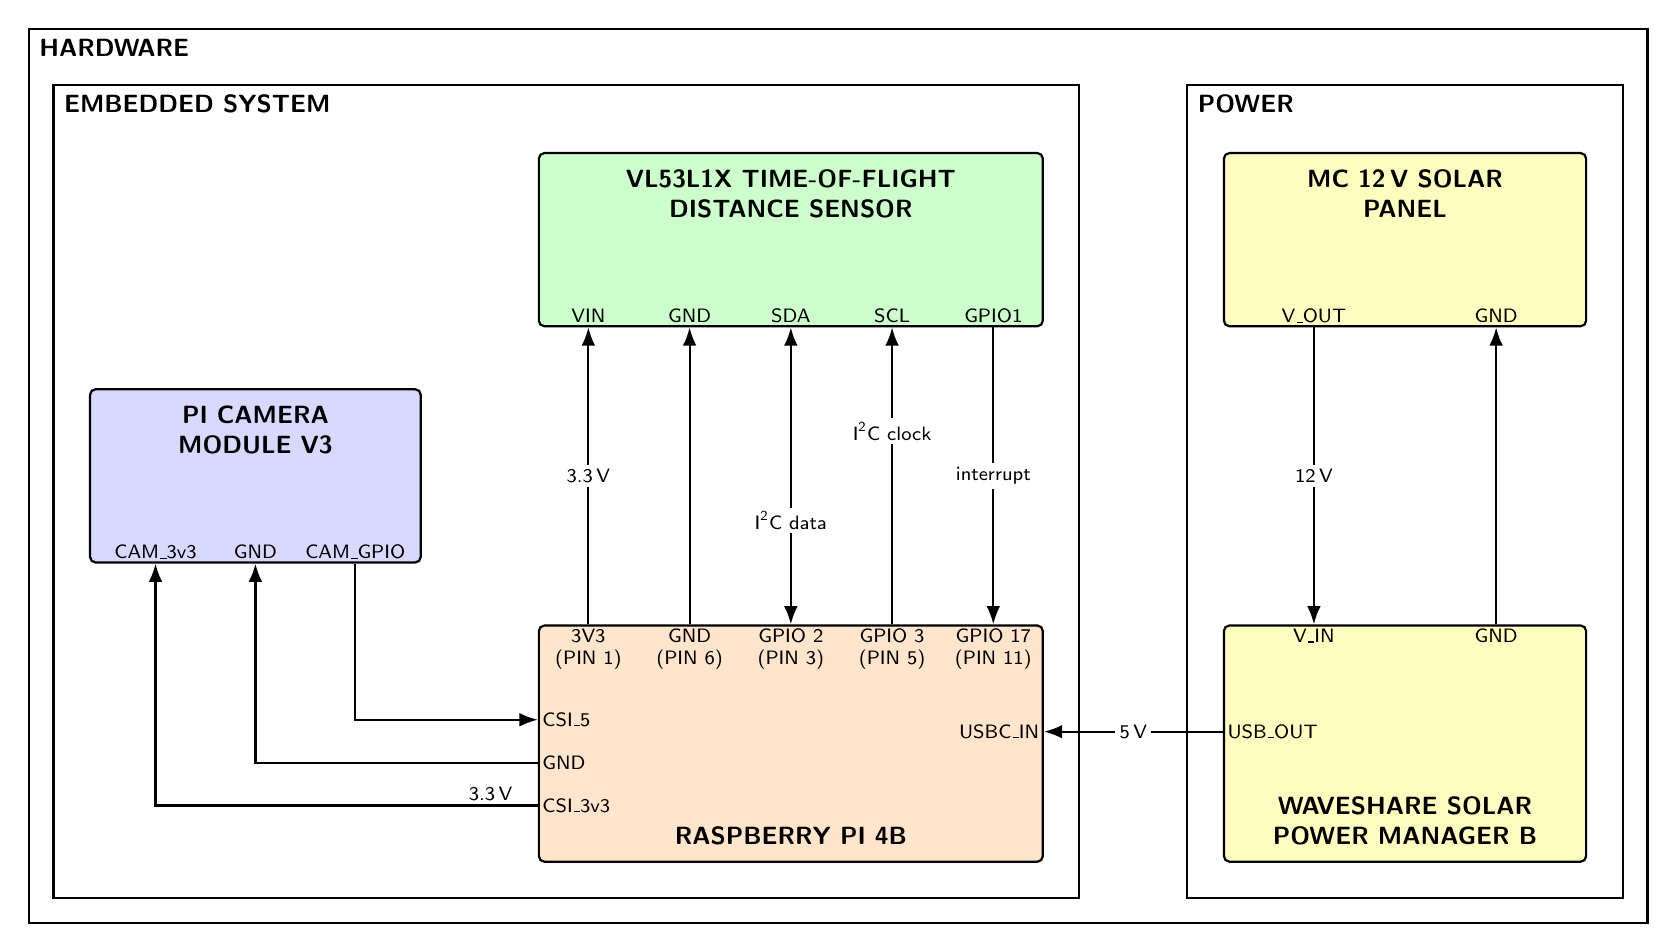
\begin{tikzpicture}[
    >=Latex,
    font=\sffamily,
    block/.style={
        rectangle,
        draw,
        thick,
        rounded corners=2pt,
        minimum height=2.2cm
    },
    camerablock/.style={block, fill=blue!15, minimum width=4.2cm},
    sensorblock/.style={block, fill=green!20, minimum width=6.4cm},
    computerblock/.style={block, fill=orange!20, minimum width=6.4cm, minimum height=3.0cm},
    powerblock/.style={block, fill=yellow!25, minimum width=4.6cm},
    title/.style={font=\sffamily\bfseries\small, align=center},
    pin/.style={font=\sffamily\scriptsize, inner sep=1.5pt, align=center},
    signal/.style={font=\sffamily\scriptsize, fill=white, inner sep=1.5pt},
    wire/.style={->, thick},
    group/.style={draw, thick, inner sep=0.45cm},
    grouplabel/.style={font=\sffamily\bfseries\small, anchor=north west, inner sep=4pt}
]

% ---------------------------------------------------------------- Blocks
\node[sensorblock]   (tof)   at (6.8,  3.2) {};
\node[camerablock]   (cam)   at (0.0,  0.2) {};
\node[computerblock] (pi)    at (6.8, -3.2) {};
\node[powerblock]    (solar) at (14.6, 3.2) {};
\node[powerblock, minimum height=3.0cm] (psu) at (14.6,-3.2) {};

% ---------------------------------------------------------------- Titles
\node[title, below=3pt of tof.north]   {VL53L1X TIME-OF-FLIGHT\\DISTANCE SENSOR};
\node[title, below=3pt of cam.north]   {PI CAMERA\\MODULE V3};
\node[title, above=3pt of pi.south]    {RASPBERRY PI 4B};
\node[title, below=3pt of solar.north] {MC 12\,V SOLAR\\PANEL};
\node[title, above=3pt of psu.south]   {WAVESHARE SOLAR\\POWER MANAGER B};

% ---------------------------------------------------------------- Pins
% ToF sensor (bottom edge)
\node[pin, anchor=south] (tofVIN) at ($(tof.south west)!0.1!(tof.south east)$) {VIN};
\node[pin, anchor=south] (tofGND) at ($(tof.south west)!0.3!(tof.south east)$) {GND};
\node[pin, anchor=south] (tofSDA) at ($(tof.south west)!0.5!(tof.south east)$) {SDA};
\node[pin, anchor=south] (tofSCL) at ($(tof.south west)!0.7!(tof.south east)$) {SCL};
\node[pin, anchor=south] (tofINT) at ($(tof.south west)!0.9!(tof.south east)$) {GPIO1};

% Camera module (bottom edge)
\node[pin, anchor=south] (cam3v3) at ($(cam.south west)!0.2!(cam.south east)$) {CAM\_3v3};
\node[pin, anchor=south] (camGND) at ($(cam.south west)!0.5!(cam.south east)$) {GND};
\node[pin, anchor=south] (camIO)  at ($(cam.south west)!0.8!(cam.south east)$) {CAM\_GPIO};

% Raspberry Pi (top edge)
\node[pin, anchor=north] (pi3V3)  at ($(pi.north west)!0.1!(pi.north east)$) {3V3\\(PIN 1)};
\node[pin, anchor=north] (piGND)  at ($(pi.north west)!0.3!(pi.north east)$) {GND\\(PIN 6)};
\node[pin, anchor=north] (piSDA)  at ($(pi.north west)!0.5!(pi.north east)$) {GPIO 2\\(PIN 3)};
\node[pin, anchor=north] (piSCL)  at ($(pi.north west)!0.7!(pi.north east)$) {GPIO 3\\(PIN 5)};
\node[pin, anchor=north] (piGPIO) at ($(pi.north west)!0.9!(pi.north east)$) {GPIO 17\\(PIN 11)};
% Raspberry Pi (left edge)
\node[pin, anchor=west]  (piCSI5)   at ($(pi.north west)!0.40!(pi.south west)$) {CSI\_5};
\node[pin, anchor=west]  (piCSIGND) at ($(pi.north west)!0.58!(pi.south west)$) {GND};
\node[pin, anchor=west]  (piCSI3v3) at ($(pi.north west)!0.76!(pi.south west)$) {CSI\_3v3};
% Raspberry Pi (right edge)
\node[pin, anchor=east]  (piUSB)    at ($(pi.north east)!0.45!(pi.south east)$) {USBC\_IN};

% Solar panel (bottom edge)
\node[pin, anchor=south] (solOUT) at ($(solar.south west)!0.25!(solar.south east)$) {V\_OUT};
\node[pin, anchor=south] (solGND) at ($(solar.south west)!0.75!(solar.south east)$) {GND};

% Power manager (top and left edges)
\node[pin, anchor=north] (psuIN)  at ($(psu.north west)!0.25!(psu.north east)$) {V\_IN};
\node[pin, anchor=north] (psuGND) at ($(psu.north west)!0.75!(psu.north east)$) {GND};
\node[pin, anchor=west]  (psuOUT) at ($(psu.north west)!0.45!(psu.south west)$) {USB\_OUT};

% ---------------------------------------------------------------- Connections
% Raspberry Pi <-> ToF sensor (I2C bus plus interrupt line)
\draw[wire] (pi3V3.north |- pi.north) -- node[signal] {3.3\,V} (tofVIN.south |- tof.south);
\draw[wire] (piGND.north |- pi.north) -- (tofGND.south |- tof.south);
\draw[wire, <->] (piSDA.north |- pi.north) -- node[signal, pos=0.35] {I\textsuperscript{2}C data} (tofSDA.south |- tof.south);
\draw[wire] (piSCL.north |- pi.north) -- node[signal, pos=0.65] {I\textsuperscript{2}C clock} (tofSCL.south |- tof.south);
\draw[wire] (tofINT.south |- tof.south) -- node[signal] {interrupt} (piGPIO.north |- pi.north);

% Raspberry Pi <-> camera module (CSI ribbon)
\draw[wire] (camIO.south |- cam.south) |- (piCSI5.west -| pi.west);
\draw[wire] (piCSIGND.west -| pi.west) -| (camGND.south |- cam.south);
\draw[wire] (piCSI3v3.west -| pi.west) -- ++(-1.2,0) node[signal, midway, above] {3.3\,V}
            -| (cam3v3.south |- cam.south);

% Solar panel <-> power manager
\draw[wire] (solOUT.south |- solar.south) -- node[signal] {12\,V} (psuIN.north |- psu.north);
\draw[wire] (psuGND.north |- psu.north) -- (solGND.south |- solar.south);

% Power manager -> Raspberry Pi
\draw[wire] (psuOUT.west -| psu.west) -- node[signal] {5\,V} (piUSB.east -| pi.east);

% ---------------------------------------------------------------- Groupings
\begin{scope}[on background layer]
    % Extra headroom above each group leaves space for its label
    \node[group, fit={(cam) (tof) (pi) ($(tof.north)+(0,0.4)$)}] (embedded) {};
    \node[group, fit={(solar) (psu) ($(solar.north)+(0,0.4)$)}] (power) {};
    \node[group, fit={(embedded) (power) ($(embedded.north)+(0,0.4)$)}, inner sep=0.3cm] (hardware) {};
\end{scope}
\node[grouplabel] at (embedded.north west) {EMBEDDED SYSTEM};
\node[grouplabel] at (power.north west)    {POWER};
\node[grouplabel] at (hardware.north west) {HARDWARE};

\end{tikzpicture}%
}
\caption{Hardware interfacing diagram of the smart sunbird feeder, showing the hardware subsystems and the power and signal connections between them.}
\label{fig:hardware_block_diagram}
\end{figure}

\subsection{Feeder and Mechanical Design}
\label{subsec:FeederMechanicalDesign}

% \begin{itemize}
%     \item Describe the nectar-feeder arrangement.
%     \item Explain bird positioning relative to the feeder and camera.
%     \item Describe the feeder mounting method and measures used to reduce sway.
%     \item Discuss accessibility for cleaning and refilling.
%     \item Consider mechanical robustness and outdoor suitability.
% \end{itemize}

As previously mentioned in Chapter~\ref{ch:LitReview} and Chapter~\ref{ch:Methodology}, sunbirds are nectar-feeding birds. The proper storage and maintainence of a nectar feeder are key considerations when selecting the feeding mechanism. The nectar is reuired to be replaced every 48 hours at most, with its container being cleaned at similar intervals to remain hygenic and safe for bird use. These requirements translate to a need for an easily-accessible feeder that is robust to environmental factors and is capable of storing liquid reliably and without risk of contamination.

Due to these intricate requirements of the feeder for this project, it was decided that this project will utilize a very simple, commercially available nectar feeder. The feeder selected for this project was chosen for its simplicity, availability, cost-effectiveness and proven satisfaction of all necessary concerns of reliability and safety. The feeder used for this project, a 750\,ml sunbird nectar feeder from Stodels \cite{StodelsSunbirdFeeder}, is shown in Figure~\ref{fig:stodels_nectar_feeder}.

\begin{figure}[htbp]
\centering
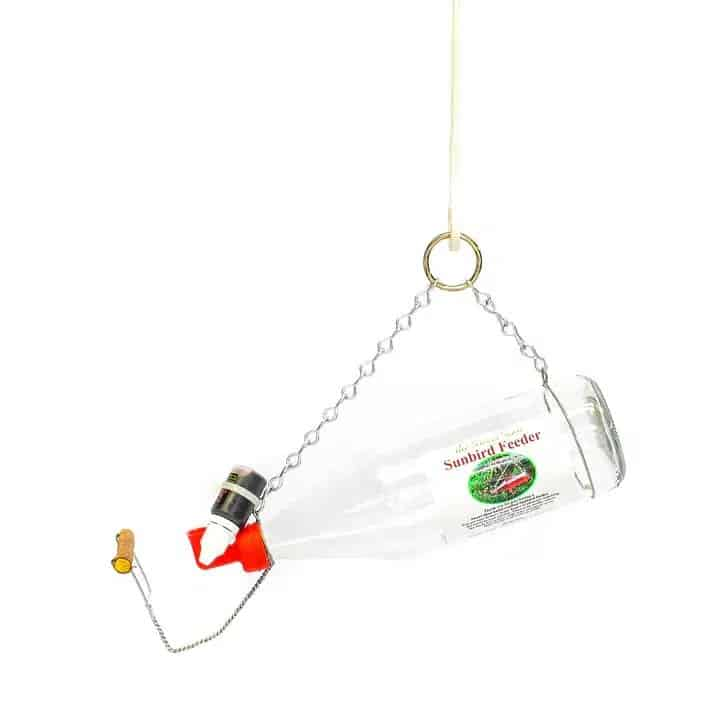
\includegraphics[width=0.4\textwidth]{3_Chapters/4_Chapter_Design/Figures/stodels_nectar_feeder.jpg}
\caption{The commercially available Stodels 750\,ml sunbird nectar feeder used in this project \cite{StodelsSunbirdFeeder}.}
\label{fig:stodels_nectar_feeder}
\end{figure}

This project required multiple additional components to be physically connected to the feeder. The stock feeder selected for this project offered little purchase for such components to be attached between its smooth glass body and minimal chain support mechanism. For this reason, it was decided to remove the chains entirely from the glass bottle and integrate the bottle into a larger housing that better accommodated for the introduction of the extra components required. The design of this housing is documented further in Section~\ref{subsec:EnclosureOutdoorDesign}.

\subsection{Embedded Computing and Camera}
\label{subsec:EmbeddedCameraDesign}

\begin{itemize}
    \item Present the selected embedded computing platform.
    \item Present the selected camera module.
    \item Describe the relevant interfaces between the camera and embedded computer.
    \item Include important technical specifications relevant to system operation.
    \item Explain how the selected hardware satisfies the processing and imaging requirements of the project.
\end{itemize}


\subsection{Visit-Detection Hardware}
\label{subsec:VisitDetectionHardware}

\begin{itemize}
    \item Describe any sensor hardware used to detect or trigger bird visits.
    \item Explain sensor positioning and connection to the embedded computing platform.
    \item Discuss relevant detection range, response and interface considerations.
    \item If visit detection is implemented entirely in software, move the relevant discussion to Section~\ref{sec:SoftwareDesign}.
\end{itemize}


\subsection{Storage and Hardware Interfaces}
\label{subsec:StorageHardwareInterfaces}

\begin{itemize}
    \item Describe the local storage hardware used by the system.
    \item Present the main electrical and communication interfaces between components.
    \item Include a simplified hardware connection diagram where appropriate.
    \item Discuss any supporting electronics required for system operation.
\end{itemize}


\subsection{Power and Solar System}
\label{subsec:PowerSolarDesign}

\begin{itemize}
    \item Present the overall power architecture.
    \item Describe the battery, solar panel, charge controller and voltage-regulation components.
    \item Explain power distribution to the embedded computer and peripherals.
    \item Include provision for manual charging where applicable.
    \item Present relevant sizing calculations or design equations where necessary.
\end{itemize}


\subsection{Enclosure and Outdoor Installation}
\label{subsec:EnclosureOutdoorDesign}

\begin{itemize}
    \item Describe the enclosure used for the electronics and power components.
    \item Explain protection against rain, moisture, dust and direct environmental exposure.
    \item Discuss ventilation and thermal considerations.
    \item Describe the mounting arrangement for the electronics, battery and solar panel.
\end{itemize}


\section{Software Design}
\label{sec:SoftwareDesign}

\subsection{Software Architecture}
\label{subsec:SoftwareArchitecture}

\begin{itemize}
    \item Present the overall software architecture.
    \item Include a software block diagram or flow diagram.
    \item Identify the main software modules and their interactions.
\end{itemize}


\subsection{Visit Detection and Video Capture}
\label{subsec:VisitDetectionVideoCapture}

\begin{itemize}
    \item Describe the software logic used to detect or respond to a bird visit.
    \item Explain how video recording is initiated and terminated.
    \item Describe how recorded visits are separated and stored.
    \item Explain the handling of repeated or false triggers where relevant.
\end{itemize}


\subsection{Video Processing and Species Identification}
\label{subsec:VideoProcessingSpeciesID}

\begin{itemize}
    \item Describe how recorded video is processed prior to inference.
    \item Explain the frame-selection method.
    \item Describe any image preprocessing.
    \item Present the selected species-classification model.
    \item Define the locally relevant classification classes.
    \item Explain inference and confidence handling.
    \item Describe how multiple frame predictions are combined into a visit-level result where applicable.
\end{itemize}


\subsection{Data Logging and Storage}
\label{subsec:DataLoggingStorage}

\begin{itemize}
    \item Describe how visit information is logged.
    \item Present the database structure at an appropriate level of detail.
    \item Describe the storage of:
    \begin{itemize}
        \item Date and time.
        \item Video file location.
        \item Predicted species.
        \item Classification confidence.
        \item Visit duration.
        \item Processing status.
        \item Relevant system logs.
    \end{itemize}
\end{itemize}


\subsection{Web Interface}
\label{subsec:WebInterfaceDesign}

\begin{itemize}
    \item Describe the local web-interface architecture.
    \item Explain interaction between the web server, database and stored video files.
    \item Present the main interface functions, including:
    \begin{itemize}
        \item Dashboard.
        \item Recent visit history.
        \item Species-identification results.
        \item Video playback.
        \item Basic system status.
        \item Relevant settings where implemented.
    \end{itemize}
\end{itemize}


\subsection{System Control and Reliability}
\label{subsec:SystemControlReliability}

\begin{itemize}
    \item Describe software mechanisms used to support reliable unattended operation.
    \item Discuss relevant features such as:
    \begin{itemize}
        \item Automatic startup.
        \item Error handling.
        \item Process recovery.
        \item Storage management.
        \item System logging.
        \item Power-aware operation.
    \end{itemize}
    \item Omit this subsection if these functions are more appropriately discussed within the preceding software subsections.
\end{itemize}


\section{System Integration}
\label{sec:SystemIntegration}

\begin{itemize}
    \item Explain how the hardware, software, mechanical and power subsystems are combined.
    \item Present the final integrated system architecture.
    \item Include photographs or annotated diagrams of the completed system where appropriate.
    \item Discuss any important integration constraints or modifications.
    \item Avoid repeating detailed subsystem descriptions already presented earlier in the chapter.
\end{itemize}


\section{Bill of Materials}
\label{sec:BillOfMaterials}

\begin{itemize}
    \item Present the main components used in the completed system.
    \item Include:
    \begin{itemize}
        \item Component.
        \item Quantity.
        \item Function.
        \item Supplier or source.
        \item Unit cost.
        \item Total cost.
    \end{itemize}
    \item Group components into mechanical, electronic and power categories where useful.
\end{itemize}

% Example table structure:
%
% \begin{table}[ht]
% \centering
% \caption{Bill of materials for the smart sunbird feeder}
% \label{tab:BillOfMaterials}
% \begin{tabular}{lclrr}
% \hline
% \textbf{Component} & \textbf{Qty.} & \textbf{Supplier} &
% \textbf{Unit Cost} & \textbf{Total Cost} \\
% \hline
% Raspberry Pi & 1 & -- & R-- & R-- \\
% Camera Module & 1 & -- & R-- & R-- \\
% Battery & 1 & -- & R-- & R-- \\
% Solar Panel & 1 & -- & R-- & R-- \\
% \hline
% \end{tabular}
% \end{table}


\section{Conclusion}
\label{sec:DesignConclusion}

\begin{itemize}
    \item Summarise the completed system design.
    \item Reinforce how the hardware and software subsystems combine into a functional smart sunbird feeder.
    \item Relate the final design back to the main system requirements.
    \item Transition to the subsequent chapter covering system testing, results and evaluation.
\end{itemize}
% Chapter 5 - Results

\glsresetall % reset the glossary to expand acronyms again
\chapter[Results]{Results}\label{ch:Results}
\index{Results}

% Results
\section[Results]{Results}
\begin{itemize}
	\item{Describe the experimental setup (ie. Hardware)}
	\item{Describe your experiments}
	\item{Describe your results}
\end{itemize}

This chapter should generally present your finding in the form of figures, tables, equations, code listings, etc. It is for presenting and discussing your findings, which can split into sections if the experiment has multiple parts, or stages.  You might also want to have a `Discussion' or `Discussion of Results' chapter, which may focus on either more detailed discussion of particular results, or more comprehensive discussion of the results and system performance as a whole.  If you have a Discussion of Results section, then you do not want to discuss too much about the specific results in this chapter and rather move the main discussion or reflective considerations of these to the Discussion of Results chapter.

However, and this is an important reminder, ensure that you do have some text of discussion for your results, to take the reader through your results and the figures you may provide.  Make sure not to just put one figure after another without any attempt to explain the sequencing and what is being shown and perhaps some key issues in the figures presented (a monolithic sequence of figure after figure without any attempt at explanation will get undesirable responses from examiners).

If you have an experiments section, it is often useful to have a clear connection of experiment section corresponding to a result section showing results for that test. Examiners often appreciate that sort of clear and consistent structure that is easy to follow.  For example, if you have section~5.1 as Modular Testing, then you could correspond to~6.1 Modular Testing Results (the two sections should be cross-linked with \verb|\label| and \verb|\ref|, in both directions)

\section{Tips for Results Figures}

Include good quality graphs (see Fig.~\ref{fig:r_vs_N_f=0_0005_P=90} for an example).

\begin{figure}[ht]
\centering
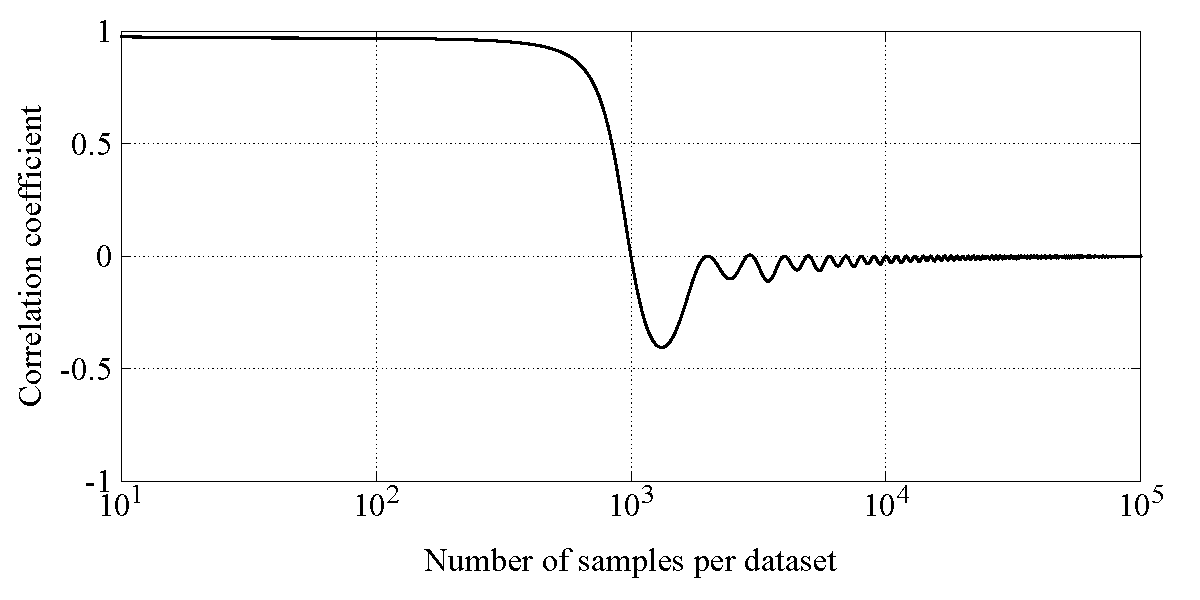
\includegraphics[width=0.8\columnwidth]{3_Chapters/5_Chapter_Results/Figures/r_vs_N_f=0_0005_P=90.pdf}
\caption{The correlation coefficient as a function of sample count}
\label{fig:r_vs_N_f=0_0005_P=90}
\end{figure}

An easy way to obtain more space for an article is to use wide, flat figures, such as Fig.~\ref{fig:Line_Signals}.

\begin{figure}[ht]
\centering
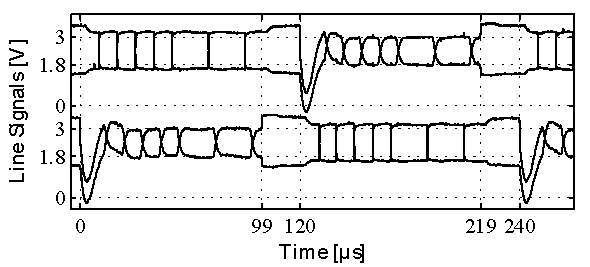
\includegraphics[width=0.8\columnwidth]{3_Chapters/5_Chapter_Results/Figures/Line_Signals.pdf}
\caption{Oscilloscope measurement showing physical line signals on both ends of a transmission line during master switch-over}
\label{fig:Line_Signals}
\end{figure}

Always remember to include axes text, units and a meaningful caption in your graphs. When typing units, a $\mu$ sign has a tail! The letter ``u'' is not a valid unit prefix. When typing resistor values, use the $\Omega$ symbol.

\section{Pictures and screenshots}

When you include screenshots, pdf\LaTeX{} supports JPG and PNG file formats.  PNG is preferred for screenshots, as it is a loss-less format.  JPG is preferred for photos, as it results in a smaller file size.  It's generally a good idea to resize photos (not screenshots) to be no more that 300~dpi, in order to reduce file size. \textbf{Never change the aspect ratio of screenshots and pictures!}

Fig.~\ref{fig:UCT.pdf} shows an example of a PDF image with custom scaling.

\begin{figure}[ht]
\centering

\includegraphics[width=0.35\columnwidth]{3_Chapters/5_Chapter_Results/Figures/UCT.pdf}
\caption{An example image with custom scaling}
\label{fig:UCT.pdf}
\end{figure}

Make sure to always use the best quality image possible.  Use JPEG for photos, PNG for screenshots and PDF (scalable vector graphics) for everything else.  JPEG is lossy, but good for photos, whereas PNG is lossless and good for images with large areas of solid colour.\\

\vspace{5mm}
\hfill
\begin{minipage}[b]{0.3\textwidth}\centering\setlength{\parindent}{0mm}

\includegraphics[width=\textwidth]{3_Chapters/5_Chapter_Results/Figures/UCT.jpg}\\%
{\small (a)~~JPEG}%
\end{minipage}
\hfill
\begin{minipage}[b]{0.3\textwidth}\centering\setlength{\parindent}{0mm}

\includegraphics[width=\textwidth]{3_Chapters/5_Chapter_Results/Figures/UCT.png}\\%
{\small (b)~~PNG}%
\end{minipage}
\hfill
\begin{minipage}[b]{0.3\textwidth}\centering\setlength{\parindent}{0mm}

\includegraphics[width=\textwidth]{3_Chapters/5_Chapter_Results/Figures/UCT.pdf}\\%
{\small (c)~~SVG}%
\end{minipage}
\hfill\mbox{}

% Chapter 6 - Conclusions

\glsresetall % reset the glossary to expand acronyms again
\chapter[Conclusions]{Conclusions}\label{ch:Conclusion}
\index{Conclusions}

% Conclusions
\section{Conclusions}
\begin{itemize}
	\item{Restate the problem. State the novel solution.}
	\item{Summarize what has been accomplished}
	\item{Summarize any limitations}
	\item{What worked really well and has a big impact?}
\end{itemize}

% Future Work
\section{Future Work}
\begin{itemize}
	\item{How do you hope to continue work on this topic?}
	\item{Are there possible extensions?}
	\item{What are some improvements that could be made?}
\end{itemize}

%*******************************************************************************
% 0.8 - BIBLIOGRAPHY
%*******************************************************************************

% Put in \nocite{*} so all entries in the bibliography are included
\nocite{*}

% Print Bibliogrpahy
\phantomsection

% Uncomment for a plain bibliography else use IEEE style below
%\bibliographystyle{plain}
%\bibliography{4_References/References}

% IEEE-style bibliography (included with standard LaTeX distributions)
\bibliographystyle{ieeetr}
\bibliography{4_References/References}

\clearpage

%*******************************************************************************
% 0.9.1 - APPENDICES
%*******************************************************************************

\appendix

% Appendix A
\updatechaptername
\chapter{Supporting Data}

Appendix sections are where you can place large figures, data tables, and spinets of code. Use appendices to your benefit to keep the body of your thesis concise!

The lyrics found below are for your enjoyment, but also serve an important role in demonstrating latex syntax for formatting text and in-text citations.  

\section{Lyrics to Soft Kitty}

\begin{center}
\mbox{}
Soft kitty, warm kitty\\
Little ball of fur\\
Happy kitty, sleepy kitty\\
Purr, purr, purr\\[0.5in]

This has been brought to you by Sheldon Cooper.
\end{center}

\clearpage


% Appendix B
\updatechaptername
\chapter{Satirical Support}

This section provides some comic relief. In addition, it serves as an example of how to insert an image into your thesis with proper caption, label and citation.

\begin{figure}[ht]
	\centering
	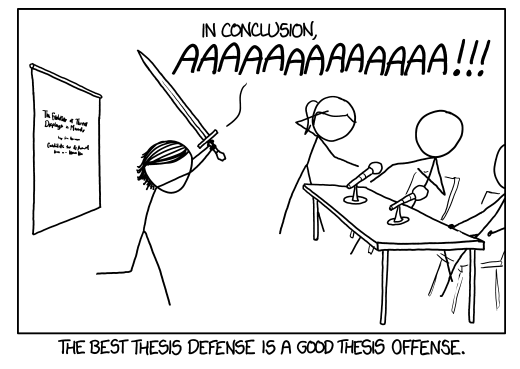
\includegraphics[width = 4.5in]{5_Appendices/Appendix_B/Figures/Thesis_Defence.png}
	\caption{You must prepare to defend your thesis.}
	\label{fig:DEFENCE}
\end{figure}

\clearpage



%*******************************************************************************
% 0.9.2 - INDEX
%*******************************************************************************
% Creates the index
% Uncomment if an INDEX should be created

% \printindex

%*************************************************************************************************************
% 1.0 - END OF DOCUMENT
%*************************************************************************************************************
\end{document}
